

\chapter{Optimal Service Replica Placement via Model Predictive Control}
\label{ch:replica_placement_through_mpc}    
%\begin{center}
%\textbf{This chapter contains material from Ghanbari et al. \cite{ghanbari2014mpc}}.
%\end{center}

This chapter presents a dynamic service placement algorithm for Optimal Service Placement (OSP) of a set of N-tire software applications. The algorithm solves an optimization problem in each control step. 
The solution of the optimization suggests some service replicas to be added or removed from the available hosts. These deployment changes are optimal with regards to overall long-term objectives. In addition, the optimization considers the restrictions imposed on the number of possible service migrations at each time interval.  

%In the second part of this chapter, we propose a technique to for finding the optimal of reservation actions to minimize cost in a public IaaS cloud environment. The problem here was to reserve enough number of hosts preemptively to accommodate the workloads. The optimality of our approach is only guaranteed if the hosts are homogeneous, that is the cloud only offers one type of resource.\footnote{Note that this differentiates this problem from the optimal selection of active hardware components.}  With more types of hosts, the optimization problem becomes an integer programming. Thus, we use a heuristic in case of multiple resource types that only achieves a sub-optimal solution.

%\begin{spacing}{1} 
% \begin{algorithm}
%        \small
%        \SetAlgoVlined
%        \SetKwInOut{Input}{input}e
%        \SetKwInOut{Output}{output}
%%        \SetKwInOut{Initialize}{initialize}
%        \SetKwInOut{Variables}{variables}  
%  \SetAlFnt{\tiny}
%\Input{desired response times regarding customer classes}
%\Output{optimal placement $u$ and reservation actions for current step }
%\BlankLine
%in each time interval: 
%  estimate workload component (N,Z,D)  and host capacity (mu)? and throughput x (if unobserved) using accurate QM. \\
%  calculate the system necessary throughput to support the workload component \\ % using N, Z translate the target R into X 
%  calculate the NFM demands (d) based on the observed/estimated throughputs, capacities ? \\
%  plan the resource reservation and/or allocation actions for current time interval  \\
%\caption{hi}
%\label{algorithm1}
%\end{algorithm}
%\end{spacing}  

\section{Problem Components}  
The definition of the OSP problem includes five components: hardware structure, software structure, workload, infrastructure cost, and QoS related Service Level Objectives (SLOs). The solution of the problem is an optimal set of placement changes at each timestep during the lifetime of a cloud provider. 
Each placement change is an addition or deletion of a service replica to or from a host in a data center. In the rest of this section, components of the problem are briefly discussed:  
  
\subsection{Hardware structure} We assume a cloud with heterogeneous resources composed of $H$\nomenclature[M]{$H$}{Number of hosts in a data center} hosts. Each host has a number of resources such as disks, random access memory (RAM), and processors. We assume there are $K$\nomenclature[M]{$K$}{Number of different types of resources in a data center (i.e. the CPU, disk, and the network)}\footnote{We use an uppercase letter to denote the number of onstances of an entity while using lowercase letters for indexing individual instances.} of these types of resources within the data center\footnote{Note that besides hosts, a data center is also composed of a network and a storage fabric. Although the theory developed here can be tailored for those as well, these resources are not addressed in this chapter. }. The multiplicity of resource $k$\nomenclature[M]{$k$}{Index of type of resource} of a host $h$\nomenclature[M]{$h$}{Index of a host}
 is denoted by $\capp_{h,k}$\nomenclature[M]{$\capp_{h,k}$}{The multiplicity of resource type $k$ of host $h$}. If the only resource under consideration is the CPU, then the multiplicity can be simply written as $\capp_{h}$. Each host resource is also associated with speed factor $\speedFactor_{h,k}$. If the only resource of consideration is the CPU, then speed factors are written as $\speedFactor_{h}$. 

\subsection{Software structure} We assume the system is composed of $S$\nomenclature[M]{$S$}{The number of services in the data center. } services. The software structure is modelled based on interactions of these services. We quantify these interactions using two sets (also elaborated in subsection \ref{sec:workload-demands-background}):  
 (i) The service demands of the services on different resource types of data center hosts. 
 (ii) The service call graph, where each edge from a caller service to a callee is labeled by the number of invocations for each execution of the caller. 

\subsection{Workload} The workload component was described in subsection \ref{sec:workload-background}. The workload component it is represented by $C$ classes of users that make use of the shared services. Each class $c$ of users is identified by: (i) it's number of consumers, $N_c$, and it's think time, $Z_c$, as discussed in subsection \ref{sec:workload-intensities-background},  (ii) the number of visits from classes to front-end services derived from CBMG is $V_{c,s}$, denoted for each class $c$ and service $s$.   

\subsection{Infrastructure cost} The infrastructure cost is  based on energy consumption  and is modelled as a function of resource utilizations. 
   
\subsection{Service level objectives} An SLO for each application (or class of users) is represented by an upper bound on the application's response time $R_{c}^\text{SLA}$ \nomenclature[M]{$R_{c}^\text{SLA}$}{SLO upper-bound on the response time of class $c$.} or lower bound on its throughput $X_{c}^\text{SLA}$.  \nomenclature[M]{$X_{c}^\text{SLA}$}{SLO lower bound on the throughput of class $c$.} 
As an example, consider a service center composed of 14 services ($S=14$), accessed by 2 classes of users ($C=2$). 
Figure \ref{fig:service_call_graph} represents the call graph of the services and 
the number of visits from the classes to services ($V_{c,s}$); 
the think times ($Z_c$) and 
the number of users ($N_c$)\nomenclature[M]{$N_c$}{Number of users in class $c$} of each class over time, and 
the invocation numbers within services ($y_{c,s}$). 
% see this http://old.nabble.com/Two-lables-on-a-node-(one-outside)-td31349791.html
\begin{figure}[htbp]
\begin{center}
 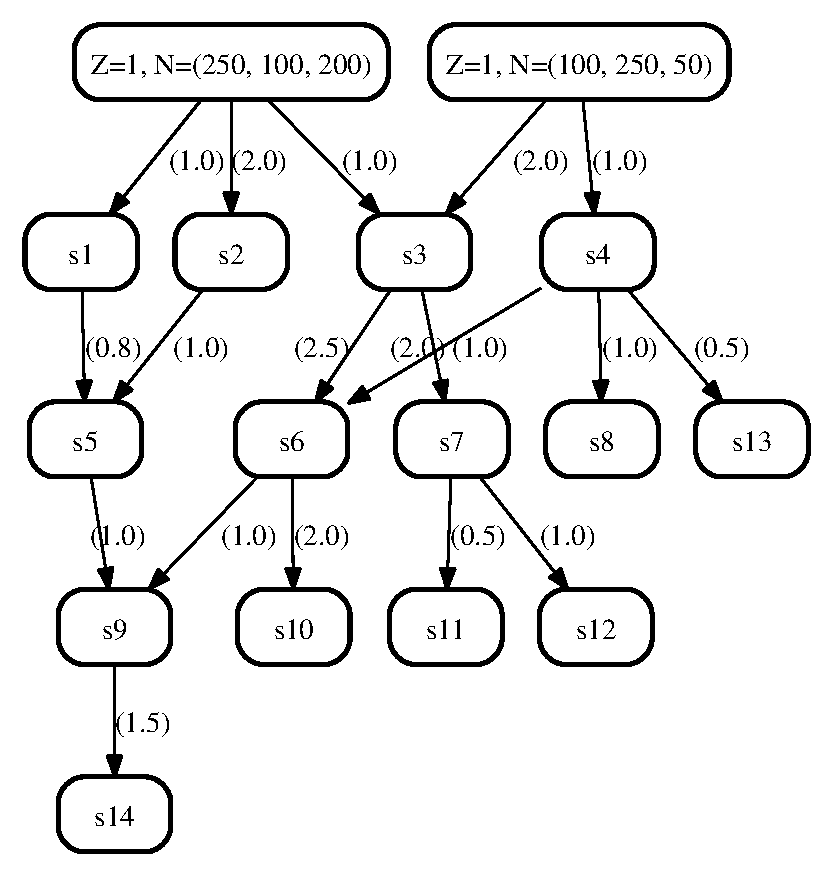
\includegraphics[scale=0.8]{image/placement/example1services}
 \caption[An example small scale service center.]{An example small scale service center: the call graph of services and classes, the number of calls from classes to services (a portion of $y$)\nomenclature[M]{$\servMeanReq_{es}$}{Mean requests made directly from any service $e$ to service $s$}, the invocation numbers within services (another portion of $y$), the think times ($Z$) and the number of users ($N$) of each class over time. }
\label{fig:service_call_graph}
\end{center}
\end{figure}
There are 6 available hosts to support the services. Capacity of the hosts are  $\capp=[16\ 6\ 6\ 16\ 6\ 6]^T$ and their CPU speed factor is $\speedFactor=[1\ 1.2\ 0.9\ 1.1\ 0.8\ 1.2]$. 
Hosts are initially unallocated, and no replica is deployed on them. % : $\theta_{s,h,0} = 0 \text{   for all $s$,$h$.}$

\section{Motivating Example}    
\label{sec:motivating-examples}   

% A Comparison of the Optimal Control and the Step-by-Step Optimization, a Hypothetical Case of a Fully Known Workload     
 In this section, using a simple example, we show the effect of solving a service placement problem using then optimal control framework. We show that if the objective is to avoid reconfiguration (i.e. there is a cost to service replication changes), and the workload has oscillations, the model predictive control provides better results than stepwise optimization. 

Consider the problem of service placement in a small-sized service center where the objective is to minimize the hosting costs and to minimize the total number of relocations while meeting the multi-class workload response time goals. 
There is a random resource cost coefficient associated with each host. The response time SLA for all the steps were set to $R^\text{SLA}_t = [0.146 \  0.267]^T$. The $R^\text{SLA}_t$ specifies the upper bound on the response time values for classes, namely $R^\text{SLA}$.

Assume a three step-ahead prediction of the mean number of users given the observations up to now ($E[N_{c,t+k}|N_{1:t}]$) is provided through some statistical prediction technique: % ; in some form such as a Dynamic Linear Model (DLM).  
% \footnote{given the fact that number of users can be non-stationary and might not have seasonal or linear trends, we could not use models such as ARIMA}:  
% The workload for this example was considered to be: 
\[
N=\left(\begin{array}{ccc} 
220.0 & 150.0 & 200.0\\ 
100.0 & 170.0 & 110.0 \end{array}\right)
\]
 where each row represents a class of users, and each column represents a future timestep. 

 The optimization was applied in two settings: (i) solving a set of individual optimizations for separate steps ignoring the transition cost (step-by-step optimization) and (ii) solving for all the steps in one optimization problem considering the cost of reconfiguration (overall optimization).            

 In the step-by-step optimization, the optimizer achieves the desired throughput by an initial deployment of 18 replicas in the first step and a total addition of 9 and removal of 11 in the subsequent steps (total changes of 38). The placements are depicted in Figure \ref{fig:stage_based_optimal_example}. 
The undirected blue dashed lines denote the placements that have been added in the corresponding steps, and the red dashed lines represent the placements that have been just removed at each time step. The black dashed lines denote the placements performed in the past time steps. 

The excessive number of service reallocations in this case are because the optimizer targets the least cost configuration (based on the host coefficients) without taking into account the cost of relocations. The removal and addition of services incur a reconfiguration cost and network overhead, and thus makes this solution suboptimal. 

Note that associating cost with the number of relocations in the current step, in case of step-by-step optimization, will not solve the problem.  This is because the effect of the relocations propagates through future steps (depending on the future workload). 

\begin{figure}[h]
\begin{center}
\subfloat[Overall optimal example][Initial placement decision (at $t=1$)]{ \includegraphics[width=0.4\textwidth]{image/placement/example1deployment_step1} \label{fig:subfig1}}  
\qquad  
%
\subfloat[Subfigure 1 list of figures text][Placement decision at $t=2$]{
 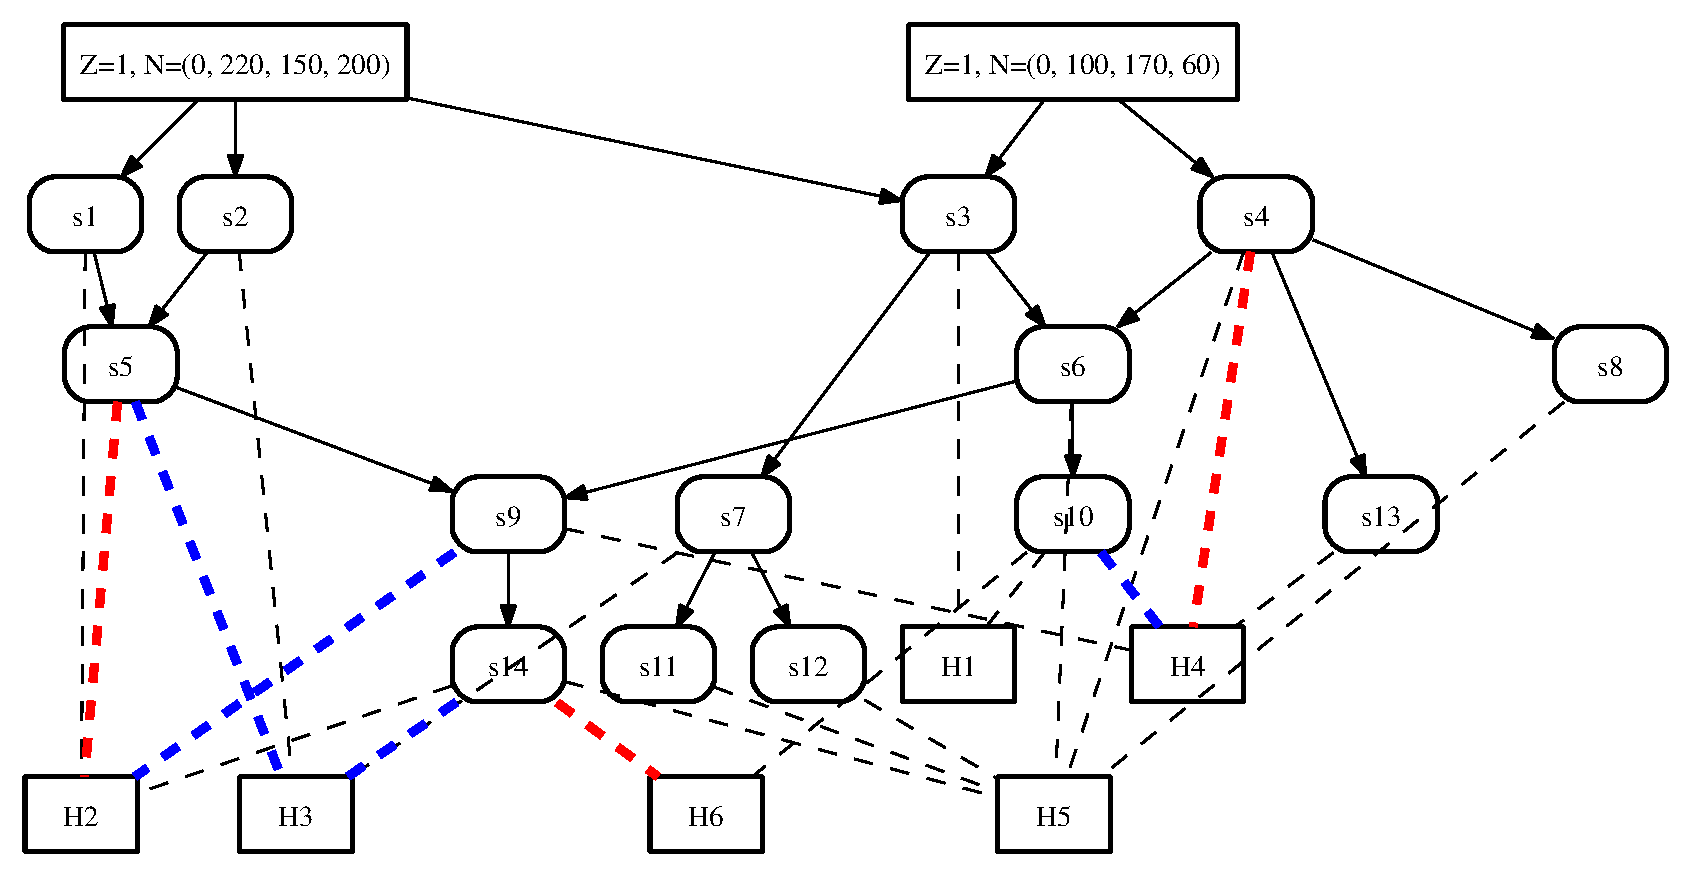
\includegraphics[width=0.5\textwidth]{image/placement/example1deployment_step2} \label{fig:subfig2}} 
  \qquad
%
  \subfloat[Subfigure 1 list of figures text][Placement decision at $t=3$]{
 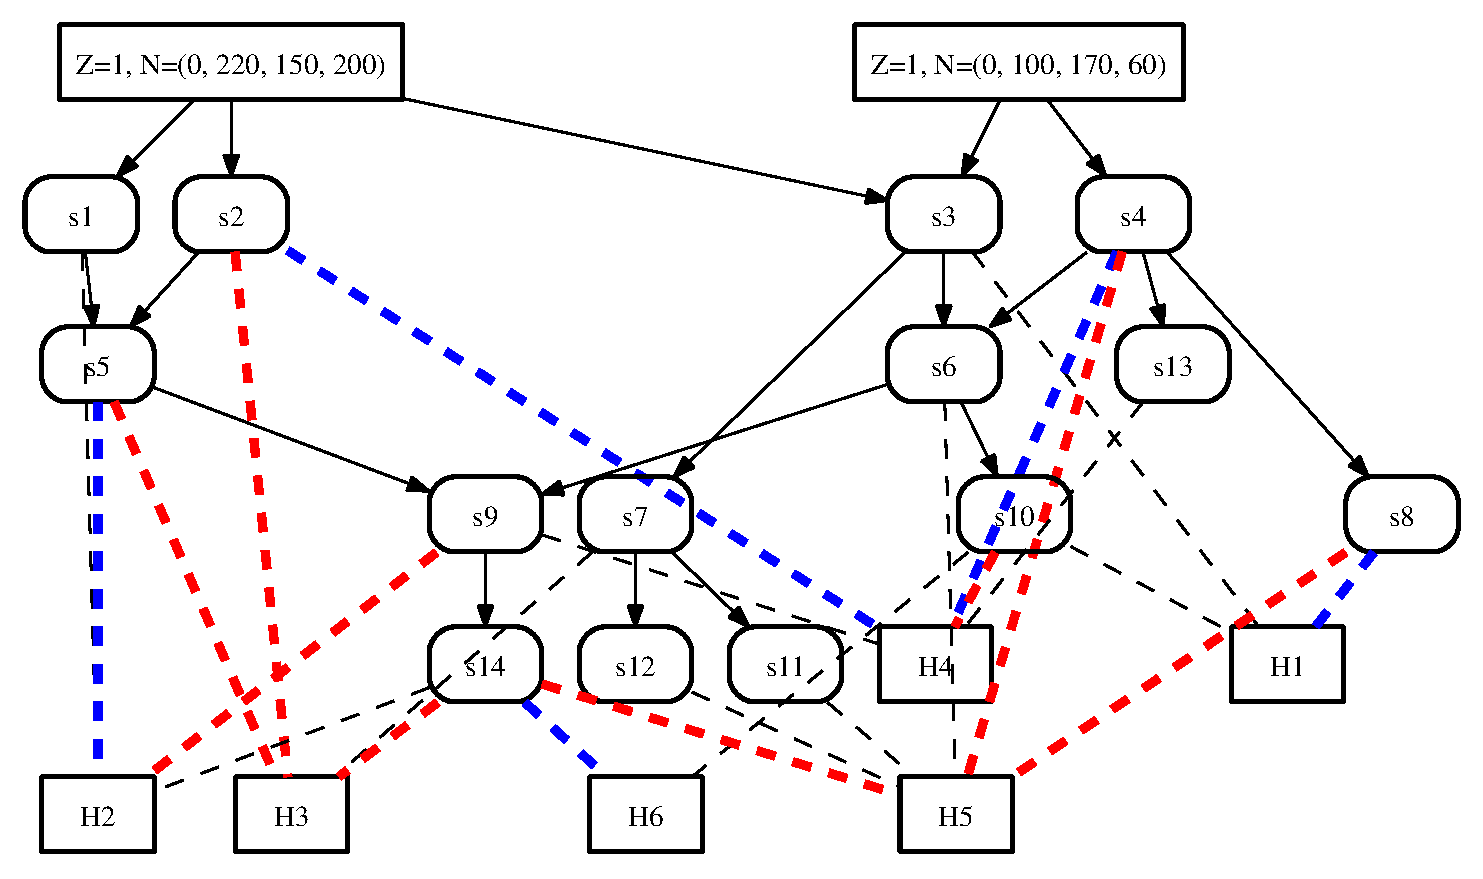
\includegraphics[width=0.5\textwidth]{image/placement/example1deployment_step3} \label{fig:subfig3}} 
 %
\caption[An example of placement decisions for a small service center using step based optimization, ignoring the future steps.]{An example of placement decisions for a small service center using step based optimization, ignoring the future steps.} 
\label{fig:stage_based_optimal_example}  
\end{center}
\end{figure}  

 In the overall optimal case, the desired throughput is achieved by an initial deployment of 19 service replicas in the first step and the total addition of 0 and the removal of 0 in the subsequent steps (total changes of 19). Although this solution is not as efficient in terms of the resource cost, 
it has a better total cost since it also considers the relocation cost. 

%The placement decisions at $t=0$ (which is maintained through $t=1$ and $t=2$) is demonstrated in Figure \ref{fig:overal_optimal_example}. 

%\begin{figure}[htbp]\begin{center}\subfloat[Overall optimal
%example][Initial placement decision (decision at
%$t=1$)]{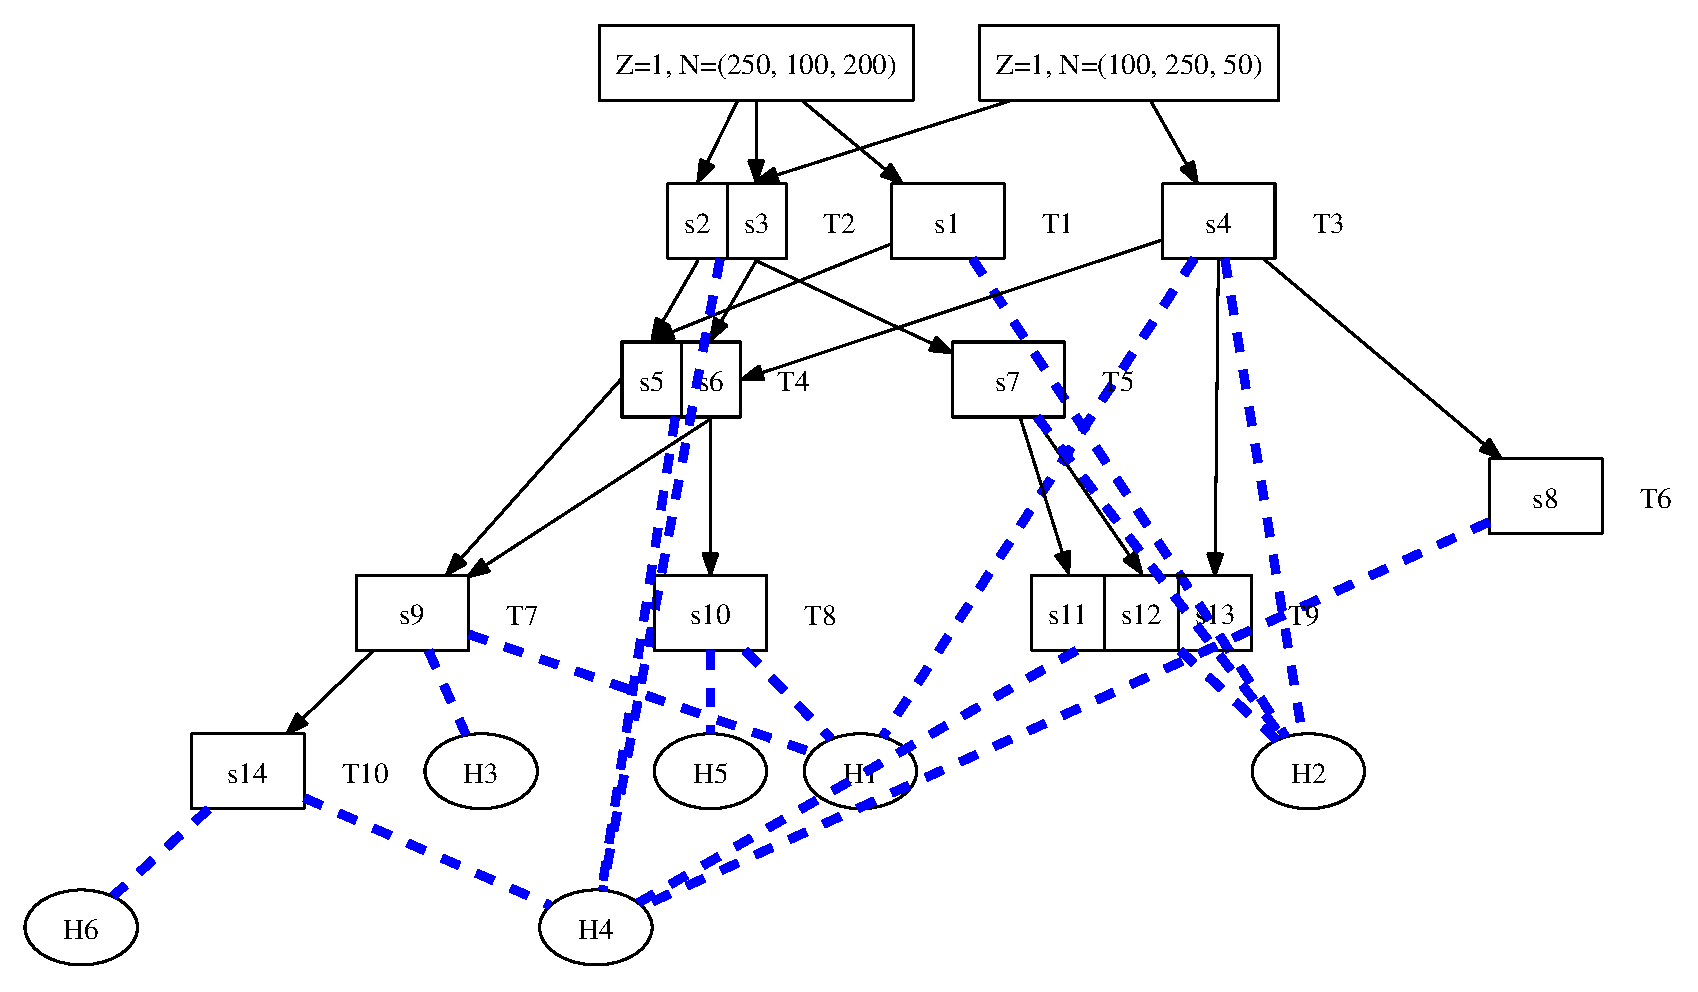
\includegraphics[scale=0.4]{image/example1deployment_overal_step1}
%\label{fig:subfig1}}
%\caption[Represents the placement decisions for a small service center
%using the optimal control.]{Represents the placement decisions for a
%small service center using the optimal control.
%}\label{fig:overal_optimal_example}\end{center}\end{figure}%

%\subsection{Example 2} 
Note that, in this example we assumed a prediction of the future mean workload conditioned on the past values is available through statistical modeling. 

% here is the example  about adding a class of service
%In this example, we show a case that a new class of services is added to the system. Consider the same small size service center. Let us assume that the system is already stabilized to the $N_{c1}=160$ users of class $c1$ with response time goal of $R^\text{SLA}_{c1}=0.146$. The class c2 joins the system at $t=1$ with a population of $N_{c2}=100$ and a SLA of $R^\text{SLA}_{c2}=1.146$. 
%The initial workload of the class of service is estimated and the load is assumed constant for the model predictive look-ahead window. Still the MPC will provide a better result than a static one-step optimization because it can distribute the necessary changes over time in a way that it better satisfies the overall objective.
	%
	%We performed a simulation of $J=100$ steps that captures the behaviour of a controlled service center until it converges to a steady-state value.   
  %
 %Figure \ref{fig:adding_class_serv_portion} shows the amount of resource given to each service, which is increased for all of the services after the 2nd class is added to the system. 
 %Figure \ref{fig:adding_class_throughput} presents the throughput of the classes. 
  %As noted  it takes around 7 steps for the throughput of the class c2 to reach its SLA value. The duration of this convergence depends on the reconfiguration cost coefficient which has been set it to $r_3=100$.  
    %
%\begin{figure}
%\begin{center}
%\subfloat[Service addition scenario, amount of resource given to each service][Amount of resource given to each service]{
 %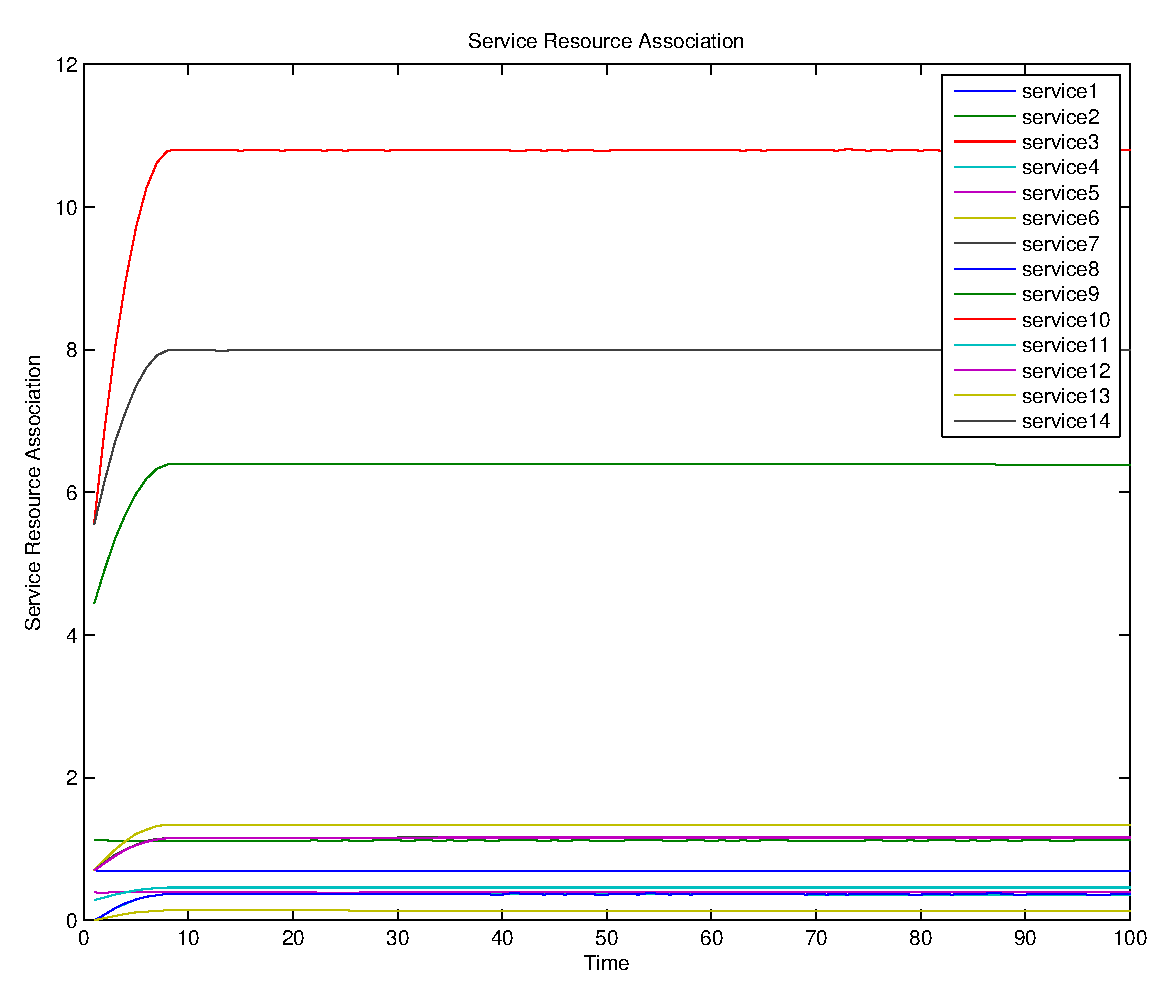
\includegraphics[scale=0.4]{image/placement/adding_class_serv_portion} \label{fig:adding_class_serv_portion}} 
  %\qquad
  %\subfloat[Service addition scenario, the throughput of classes][ the throughput of classes]{
 %\includegraphics[scale=0.4]{image/placement/adding_class_throughput} \label{fig:adding_class_throughput}} 
%\caption[Placement controller response to arrival  of a new class  of users]{Placement controller response to arrival  of a new class  of users. }
%\label{fig:stage_based_optimal_example}  
%\end{center}
%\end{figure}
     
\section{Problem Formulation}  
\label{sec:problem-formulation}  
  Having the above set of inputs, we can formulate the problem as follows:    
 assume a three-dimensional array or tensor $\theta$, whose elements are denoted by $\theta_{s,h,t}$, represents the placement of the replicas of the services on the available hosts over a time horizon\nomenclature[M]{$t$}{The timestep index}.
 In fact, each $\theta_{s,h,t}$ denotes the portion of service $s$ that is allocated to a host $h$ through a placed replica and a proper routing at a time $t$. As a result, we have: 
 \begin{align} 
&  \sum_{h=1}^H \theta_{s,h,t} = 1 & \qquad \text{for each $s$ and $t$} \label{eq:thata_totals_to_one}   
 \end{align}     
 In other words, at each time step $t$, $\theta$ represents a $H\times S$ bipartite graph  of the associations between the hosts and the services. 
 The actual demand on each resource is obtained by taking into account this association of the services and the hosts ($\theta_{s,h,t}$) \nomenclature[M]{$\theta_{s,h}$}{The portion of service $s$ that is handled by host $h$ through a placed replica and proper routing.} as:
 \begin{align} 
      %  &  d_{c,s,h,t} =  
 d_{c,s,k} \theta_{s,h,t}			\qquad & \text{for each $c$,$s$,$h$,$k$,$t$  }    
	 \label{eq:thata_as_proportion}   
 \end{align} 
  %    here $d_{c,s,h,t}$
  This expression gives the demand of class $c$ on a resource type $k$ of a server $h$  through service $s$ at time $t$, and $\theta_{s,h,t}$  denotes the portion of service $s$ that is associated to host $h$ through a placed replica and proper routing. 
 Focusing only on the CPU resource, one can drop the index $k$ representing the resource type from $d_{c,s,k}$, for simplicity. 
 For service $s$, a desired $\theta_{s,h,t}$ at time $t$ can be achieved by dividing the service invocations made to $s$ between its service replicas proportional to $\theta_{s,h,t}$ (taking $h$ as the variable):  
   \begin{align}
    y_{e,s,h} =   \theta_{s,h,t}  y_{e,s} 
   \end{align}
   where $y_{e,s,h}$ denotes the call multiplicity from each service $e$ to a replica of $s$ on $h$. $\theta_{s,h,t}$ is, in fact, the proportion of the service $s$ requests routed to its replica on the host $h$ at time $t$. 
	If for some $s$ and $h$, $\theta_{s,h,t}=0$, then there will not be any replica of service $s$ on host $h$ at time $t$. Thus, $\theta$ represents both the deployment and the quantity of resource allocation. 
 
  The cost to a cloud provider depends on the number of active hosts utilized over the providers' lifetime. The fewer active hosts used, the less cost will be incurred. 
  Indirectly, the cost depends on the placements during the provider lifetime (i.e. $\theta_{0},...,\theta_T$)\nomenclature[M]{$\theta_t$}{Placement of services on hosts at timestep $t$.}, where the provider lifetime is denoted by $T$\nomenclature[M]{$T$}{A lifetime of a cloud provider in the context of a control problem (possibly infinite).}.  

 The problem is choosing a sequence of optimal placements $(\theta^*_0,...,\theta^*_T)$ that minimizes the long term resource cost while trying to satisfy the SLOs over time. In summary, the problem is the optimal deployment of the service replicas on the available hardware over time: 
\begin{equation}
  \begin{aligned}
\underset{\theta_0,...,\theta_{T-1}} {\text{minimize } } 
   E \Bigg[ 
		 &\rSLA \sum^{T}_{t=1} \sum^C_{c=1}   \lambda_\text{SLA}(R_{c,t} - R_c^\text{SLA})   \\
   + & \rResource \sum^{T}_{t=1} \sum_{h=1}^H \lambda_{\text{resource},h}(U_{h,t})  \\
   + & \rDeployment  \sum^{T}_{t=1} \sum^H_{h=1}  \sum^S_{s=1} \lambda_\text{dep}(\theta_{s,h,t},\theta_{s,h,t-1}) \Bigg]  \\ 
\text{subject to:} \nonumber \\ 
 & R_{t} =  \text{LQM}_{\Omega,\speedFactor}(d_{t},\theta_{t}, W_{t})  &  \forall t  \\ 
 &  \sum_{h=1}^H \theta_{s,h,t} = 1 &  \forall s , t
\label{eq:opt-overall-abstract}
    \end{aligned}
\end{equation}

%
\nomenclature[M]{$\lambda(\alpha_t)$}{The cost of resources at time $t$.}
\nomenclature[M]{$u_t$}{Change in the placement made at time $t$.}  
\nomenclature[M]{$E[...]$}{An expected value.}   
\nomenclature[M]{$J_2$}{The cost of cloud provider, containing both costs of infrastructure and SLA violation.}    
Here, $T$ denotes the service centre lifetime. $(u_0,...,u_{T-1})$ is the service placements performed during this lifetime. $E\left[...\right]$ represents an expected value. $\rSLA$, $\rResource$, and $\rDeployment$ respectively represent the coefficients associated with the cost of violating SLAs, the cost of hardware resources, and the cost of changes in the deployment of services. These coefficients ($\rSLA$, $\rResource$, and $\rDeployment$) are used to tune the trade-off between the different cost factors. The expression $\lambda_\text{SLA}(R_{c,t} - R_c^\text{SLA})$ represents the cost of violating the SLO for a class $c$ at time $t$. 
Note that the SLO is defined only based on the response time of the class $c$ at each timestep (i.e., $R_{c,t}$).  
$\lambda_{\text{resource},h}(U_{h,t})$  represents the cost incurred by a host $h$, where the cost of a resource is calculated based on its utilization.
The expression $\lambda_\text{dep}(\theta_{s,h,t},\theta_{s,h,t-1})$ represents the cost of modifications in the deployment, and is calculated based on the modifications at each time step $t$. 
 Here, 
  $R_t = [R_{c,t},...,R_{c,t}]^T$ denotes the response times of the user classes over time, 
  $d_{t}$ denotes the set of service demands of the classes on the services (i.e. the matrix $(d_{c,s,t})$) for each $t$,  
 $W_t$ is the non-stationary stochastic workload of classes (i.e. $W_t = [W_{1,t},..., W_{c,t}]^T$)\nomenclature[M]{$W_0$}{Workload component composed of intensities, think time, and demands for classes at time $t$}. 
 The three cost functions ($\lambda_\text{SLA}$, $\lambda_{\text{resource},h}$, and $\lambda_\text{dep}$) are described in detail in the subsection \ref{sec:cost-elements}.  

\subsection{Equality Constraints} 
 The first equality constraint is an output equation which models the QoS attributes. Here, the QoS attributes are the response times for the classes of users (i.e. $R_t$). $R_t$ is the result of the current deployment $\theta_{t}$, the workload $W_t$, the software structure ($d_{t}$) and the structure of the data center ($\Omega$ and $\speedFactor$).
 
 Note, here we assume that the control interval is large enough that system stabilizes at each step, and, as a result, we can ignore the transient queuing dynamics and use the MVA of queuing networks to derive the output equation. Thus, the workload values are directly fed into the output equation.  
 % \footnote{Memory less systems only rely on present input rather than on all its previous values.  Let x(t) be system input, and y(t) the system output. a memory less system is denoted by:$y(t) = f(x(t))$. For systems with memory $y(t) = \int f(\tau)x(\tau)d\tau$ (integral from 0 to t), that is, the system output at the moment t depends not only on x(t), but also but also on all previous values of $x$.}:   
% and assume that $W_t$ has autonomous linear dynamics: 
% 

  \subsection{Cost elements}  
  \label{sec:cost-elements}
     In the optimization problem, to model the SLA violation cost, the function $\lambda_\text{SLA}$ is directly applied to the response time deviation of each class. The definition of $\lambda_\text{SLA}$ is as follows: 
    \begin{align} \label{eq:placement-sla-cost}
  		\lambda_\text{SLA} (x)=max\{x,0\} 
		\end{align}
  and it is a convex and increasing function. Applying this function to $(R_{c,t} - R_c^\text{SLA})$ means we desire to impose a cost whenever the response time for a class  exceeds its target SLA.
 In other situations where other behaviours are expected, $\lambda_\text{SLA}$ can be redefined using other convex functions. \nomenclature[M]{$pos(x)$}{Positive value of a real number or $max\{x,0\}$.}    

 The total cost of deployment in a data center is comprised of the cost of electricity consumed by its physical machines. The function $\lambda_\text{resource}(U_{h,t})$ is derived from the model of electricity consumption of the host. It is defined as: 
  \begin{align} \label{eq:placement-infra-cost}
  \lambda_{\text{resource},h}(U_{h,t})=  \left\{ 
  \begin{array}{l l}
   \sigma_h U_{h,t} + \sigma'_{h}  & \quad  \text{for $U_{h,t}\in (0,\Omega_h]$} \\
    0 & \quad  \text{for $U_{h,t}=0$} \\        
  \end{array} \right. 
   \end{align} 
 \nomenclature[M]{$c_h$}{A host specific cost coefficient based on utilization.}
where $\sigma_h$ and $\sigma'_h$ are host specific constants.  
 An active server with a minimum load consumes roughly 50\% of the electricity of a fully loaded server. In addition, if we model the standby servers, with an absolute zero load, the resulting cost function will have a discontinuity at the $0$ load ($U=0$).  
 This suggests that a minimum cost associated with a data center can be achieved by consolidating all the workloads in a minimum number of active machines. 

  The function $\lambda_\text{dep}(x,y)$ represents the cost of deployment changes. It is defined as the sum of the additions or removal of the service replicas to the hosts:    
\begin{align}  \label{eq:placement-trashing-cost}
& \lambda_\text{dep}(\theta_{s,h,t-1},\theta_{s,h,t})= 
& \begin{cases} 
1, & (\theta_{s,h,t}\neq0 \oplus \theta_{s,h,t-1}\neq0)  \\ 
0, & \text{otherwise} \end{cases} 
\end{align} 
where $\oplus$ denotes the logical Xor. 
$\lambda_\text{dep}(\theta_{s,h,t-1},\theta_{s,h,t})$ is 1 in two cases: (i) if the service $s$ was deployed at time $t-1$ on the host $h$ and is not deployed there at $t$, (ii) if the service $s$ was not deployed at time $t-1$ on the host $h$ and is deployed there at $t$.


 \section{A Fast Solution through MPC}   
 \label{sec:fast-solution-through-MPC} 
There are several subtleties with the form of the proposed problem. In the following subsections, we discuss each and provide a solution. 
 
\subsection{Dealing with the Non-linearity of the LQM}
The first subtlety in solving the described allocation problem is that the output equation of the system dynamics uses a nonlinear function, namely the LQM. Modelling the response times of the user classes needs a non-linear set of equalities. The LQM is an iterative algorithm for which there is no closed form general solution available.   % The first challenge is to find a way to approximate the LQM using a linear function.

 To address the non-linearity of the LQM, instead of directly using the LQM, we use its derived performance bounds. First, consider the following inequality from Queuing Networks Models (QNM): 
 %  We model the hardware constraints through the following equation:
  \begin{align} 
   \utilization_{h,k}  <  \capp_{h,k}  & \   \forall h,k \label{eq:util-capacity-inequality}
\end{align}
 \nomenclature[M]{$\utilization_{h,k}$}{Utilization of a resource $k$ of a host $h$} 
  The inequality \ref{eq:util-capacity-inequality} states that the capacity of a resource can be used as an upper bound to its utilization\footnote{Note that here we used the utilization in a slightly different way than in queuing theory. In fact, to obtain the utilization in the queuing theory sense, what we refer to as utilization here should be divided by the resource multiplicity. In the original queuing theory formula $U\leq 1$.}. Inequality \ref{eq:util-capacity-inequality} is an implication of the queuing theory and holds regardless of the type of workload to be applied to the system (open or closed). 
	
 Also, consider the following equation, derived from queuing theory, which relates utilization of resources to the throughput of user classes:    
 \begin{eqnarray} \label{eq:utilization-law-theta}
    \utilization_{h,k,t}   
    = & \sum_{c=1}^C \left(X_{c,t}  \sum_{s=1}^S (d_{c,s,k}\theta_{s,h,t})\right)  & \  \forall h,k,t    
			%  U_k = \sum_c X_c \frac{d_{c,k}}{\speedFactor_k} 
   \end{eqnarray}        
  
 This equation is derived from the equations \ref{sum-demands-on-software} and \ref{eq:thata_as_proportion}.

 Using equation \ref{eq:utilization-law-theta}, we rewrite the inequality \ref{eq:util-capacity-inequality} regarding the physical constraints as: 
   \begin{align}
   \label{eq:util-capacity-inequality2}
   \utilization_{h,k,t}   =     \sum_{c=1}^C \sum_{s=1}^S   X_{c,t} d_{c,s,k} \theta_{s,h,t}    < \capp_{h,k}  & \  \forall h,k,t
	%\[\sum_c X_c d_{c,k} < \capp_k \speedFactor_k \] 
    \end{align}  
Inequality \ref{eq:util-capacity-inequality2} is concerned with the heavy load (or saturation) situation.  
It states ``each hardware component limits the maximum possible throughput that the system can achieve. Since the bottleneck center is the first to saturate, it restricts the system's throughput most severely"\cite{lazowska1984quantitative}.

It is important to note that in case of a lightly loaded (non-saturated) system, there is another tighter upper-bound for throughput. 
``The largest possible throughput for a lightly loaded system occurs when each additional request is not delayed at all by any other requests in the system. In this case for each class $c$, no time is a spent queuing, $d_c=\sum_{h=1}^H \sum_{k=1}^K \sum_{s=1}^S d_{c,s,k} \theta_{s,h,t}$ time units are spent in service, and $Z_c$ time units are spent thinking, so the each class throughput is $N_c/(Z_c+d_c)$"\cite{lazowska1984quantitative}.
 The upper bound can thus be derived from the following equation:
   \begin{align}
   \label{eq:natural-throughput-upper-bound}
X_{c,t}\leq N^{\text{pred}}_{c,t}/\left(\sum_{h=1}^H \sum_{k=1}^K \sum_{s=1}^S d_{c,s,k} \theta_{s,h,t} +Z_c\right) 
  \end{align}    
		This throughput upper bound, however, is not our concern, because with the assumption that the response time SLAs are valid (i.e. more than the sum of service demands), the throughput SLAs will be naturally less than this upper-bound and the controller always tries to only meet this SLA; it would not waste resources and exceed the SLA when it does not reduce the cost. 

 %\subsection{Encoding the Response Time SLOs as Throughput Constraints}        
   We also need to describe the response time SLOs ($R_{c}^\text{SLA}$) in terms of throughput constraints. 
 This is done based on the assumption of finite user populations. If $N^{\text{pred}}_{c,t}$ and $Z^{\text{pred}}_{c,t}$ can be predicted and target response time $R_{c}^\text{SLA}$ is given, then the constraint based on the response time (i.e. $R_{c,t} < R_{c}^\text{SLA}$) can be translated to a constraint in terms of the throughput as:
%\begin{eqnarray}  
%R_{c} &< R_{c,SLA} & \text{for each $c$} \nonumber\\
%N_c &< N_{c,SLA}   & \text{for each $c$} \nonumber\\
%X_c &=N_c /(R_c +Z_c ) & \text{for each $c$}\\
%\end{eqnarray}  
% before encoded as 
\begin{align}
	& X_{c,t}^\text{SLA}=N^{\text{pred}}_{c,t}/(Z^{\text{pred}}_{c,t}+  R_{c,t}^\text{SLA})  & \forall  c,t  \label{eq:throughput_based_on_prediction}  \\ 
%& N_{c,t} < N_{c}^\text{SLA}   & \forall c,t \nonumber  \\ 
%& X_{c}^\text{SLA}(\vec{N})=N_{c,t}(\vec{N})/(Z_c+R_{c,t}^\text{SLA}(\vec{N}))  & \forall c,t \label{eq:convert-response-time-SLA-throughput}  \\ 
& X_{c,t}>X_{c,t}^\text{SLA}  & \forall c,t 
\end{align}
where $N^{\text{pred}}_{c,t}$ denotes the predicted mean number of users of a class $c$ at a future time $t$ and $Z^{\text{pred}}_{c,t}$ denotes the predicted mean think time of the users of a class $c$ at a future time $t$.  
Note that, the equation \ref{eq:throughput_based_on_prediction} can be calculated in advance, and the resulting $X_{c}^\text{SLA}$ can be used in several optimizations over time. 
 
\subsubsection{Approximating the Effects of Resource Contention} 
In order to derive a fast solution, we neglect the effect of the resource contention resulting from the stochastic think times and the service demands. 
In the presence of random think times (in a case of a closed workload) and random arrival rates (in the case of an open workload) queues build up at resources. We refer to this queue build-up as the hardware contention. This contention reduces the classes throughputs, increases the response times and might even shift the bottleneck from one resource to another. 
Instead of evaluating the effect of contention, we try to move the system into a region where the effect of the contention is minimized.
Usually contention happens where resources are highly utilized. Keeping the system in a region where its resource utilizations are controlled (usually between \%58 to \%80 of the capacity $\capp_h$) is a common way to avoid contention\footnote{This is sometimes referred to as the headroom principal \cite{kalyvianaki_self-adaptive_2009}.} \cite{abdelzaher_performance_2002}.  
%Formally speaking, from the equations \ref{eq:queuing-model2} and \ref{eq:queuing-model3}, we have: 
% \begin{align} 
%  X_c(N)=\frac{Q_{c,k}(N)}{(1+Q_k(N-1_c))}  \capp_k/d_{c,k} 
% \end{align}  
%  where $\frac{Q_{c,k}(N)}{(1+Q_k(N-1_c))} \capp_h$ can be considered as the portion of hardware capacity that is associated to the class $c$.
%  Note that with an assumption that the arrival of requests is deterministic, rather than being random according to a Poisson distribution, it can be deducted that  $(1+Q_k(N-1_c))  \equiv Q_k(N)$. In addition, it can be shown that this result also applies to a lightly loaded system. Thus guaranteeing the system resources are utilized under a certain threshold, we can assume that the capacity linearly contributes to the throughput (as opposed to being wasted due to the contention). 
  Thus, the inequality \ref{eq:util-capacity-inequality} might appear in the final optimization as: 
\begin{align}
 U_{h,k} \le  L \capp_{h,k}  & \  \forall h,k 
\end{align} 
where $L$ is a constant usually set to the value between 0.6 and 0.8. 

\subsection{Non-linearity in the Resource Cost}
The function $\lambda_\text{resource}$ introduced in the equation \ref{eq:placement-infra-cost} is nonlinear Because it has a discontinuity at $U=0$ (i.e. when and a physical machine is in standby mode). 
We approximate this function, based on the utilization law of the equation \ref{eq:utilization-law-theta} as:
 \[
	 f(h)=\sum^S_{s=1}  \sigma^*_{s,h} \sum_{c=1}^C X_{c,t} d_{c,s} \theta_{s,h,t}
\]
Where each  $\sigma^*_{s,h}$ is a cost coefficient. 
This cost coefficient can be based on the original values of $\sigma_{h}$ and $\sigma'_{h}$. 
For example \cite{li_fast_2009} derives similar coefficients through linear approximation of the original resource cost function.
The coefficients $\sigma_{h}$ and $\sigma'_{h}$ can be also based on some heuristics for example system administrator's preferences.
For example, for our cases studies, we used the following formula to derive $\sigma^*_{s,h}$: $\sigma^*_{s,h}=rand_{H,1}*\textbf{1}_{1,S}+10$.
In this formula, $rand_{H,1}$ are sampled from a random variable with the uniform distribution, $U(0,1)$.
% In cases studies these the values of matrix $(\sigma^*_{s,h})$ are selected in a way that the hosts with a less final cost would have less random service costs associated with them. 

  Also note that, the degree of the sparsity of the solution, and sometimes the convergence of the optimization depends on the way the elements of $\sigma^*_{s,h}$ are generated. We realized that to guarantee the sparsity in our solution it is mandatory to have different cost coefficients for different physical machines. 
 
% An important point is that the sparsity of the solution depends on the algorithm used to solve the optimization problem. Simplex method results into a sparse solution but interior point method results in a dense one. 
% 
% In a dense deployment, from each service there exists a replica on each host. %This is not certainly, what is desired since it has a lot of management overhead associated with monitoring and configuration of the service replicas. It also results into thousands of service replicas deployed on each host, which is not desired because of the context switching and the memory constraints on the service' processes.
 % Moreover, using host specific costs one can penalize the deployment of certain replica on certain host. This is for example useful in situations where installing new replicas in specific locations generates performance \footnote{for example due to cost of providing consistency where replicas are placed in distant geographical locations} or security concerns. %  this can be viewed as breaking the synchrony. 


\subsection{Nonlinearity in the Reconfiguration Cost} 
 Let us assume service placements $(\theta_{0},...,\theta_T)$ are outcomes of a process driven by a set of placement actions $(u_0,...,u_T)$. 	\nomenclature[M]{$u^*_t$}{Optimal placement action at time $t$}
 We assume that $\theta_t$ is simply a discrete-time integral (or accumulation) over the placement actions:
 \begin{align} \label{eq:placement-changes-difference}
  \theta_t = \theta_{t-1} +  u_t   
  \end{align}     
Equation \ref{eq:placement-changes-difference} represents the dynamics of the placement or the state transition.  
 Note that $\theta_{t}$ is solely driven by the placement decisions ($\{u_0,...,u_{T-1}\}$) deterministically (i.e., service center is fully predictable). The constraints resemble an ordinary difference equation with $\theta_{t}$ as a state. 
	We redefine the reconfiguration cost of equation \ref{eq:placement-trashing-cost}, over the placement decisions ($\{u_0,...,u_{T-1}\}$) using the following stage cost function:
	\begin{align}
	\lambda_\text{dep}(\theta_{s,h,t-1},\theta_{s,h,t}) =|u_{s,h,t} |
	\end{align}
	% The way this function is defined, directly affects the behaviour of the controller. In this paper, we define it as a square of $x$ (i.e. $x^2$), and sometimes as an absolute value of $x$, (i.e. $|x|$). 
	% A square function penalizes the sudden changes in the control inputs. In our formulation, this means penalizing the sudden changes in the deployment; an adaptation to address a sudden change in a workload or a SLO, has to be distributed over the time. If the cost function is defined using an absolute value, then 


\subsection{Considering the Stochastic Workload }  
\label{sec:addressing-stochastic-workload}
 Finally, to solve the abstract stochastic planning problem of Section \ref{sec:problem-formulation}, %\ref{eq:opt-overall-abstract}
 we converted it into several step-by-step deterministic optimizations over the cloud lifetime. Each optimization takes place on arrival at each new step by taking the current state as an initial point of planning.  
Further, in each optimization, the planning is only done for a limited number of future steps, which is referred to as the  \textit{lookahead horizon} and denoted by $J$; thus reducing the number of steps involved in the optimization from $T-t$ to $J$ (i.e., this assumes that $J << T-t$). 
The stochastic workload is also considered. % $E[N_{c,t+k}|N_{1:t}]$
At each time-step $t$, workloads within the lookahead horizon ${\{W_j\}}_{t\leq j \leq J}$ are fixed at their predicted conditional mean value (i.e., $E[W_j|W_{1:t}]$) based on a Dynamic Linear Model (DLM)\cite{zheng-integrated-2011}. 
Then, at each step, a perfect information\footnote{In a perfect information control problem the value of all the state variables are known (either observed or have been estimated).}, deterministic optimal control problem with a limited horizon is solved once, and the control value to be applied is derived \footnote{In original MPC this value is the first value of the planning sequence.}; everything is repeated once a new observation is available. 
% Our adapted version of CEC is presented in algorithm \ref{algorithm1}.   
The deterministic optimal control program, solved at each step, is represented in Figure \ref{fig:mpc_optimization_problem}. We describe further details of this program below. 

\begin{figure}[h!]
%\begin{spacing}{1} 
%\begin{eqnarray*} 
%\begin{aligned}
\begin{align*}
  \text{given: }   
  &  R_{c,j}^\text{SLA}\ \forall c\forall j, 
    \theta_{s,h,0}\  \forall s,\forall h,  
   \capp_{h}\ \forall h,  \\
  &  t,J,\rResource,  \rDeployment, \rSLA  \\   
  \underset{u_0,...,u_{t-1}} {\text{minimize } } 
	  & \rSLA \sum^{J}_{j=t} \sum^C_{c=1}  pos(X_{c,j}^\text{SLA}-X_{c,j})  \\
  + & \rResource \sum^{J}_{j=t} \sum^H_{h=1} \sum^S_{s=1}  \sigma^*_{s,h} \sum_{c=1}^C X_{c,j} d_{c,s} \theta_{s,h,j}   \\ 
  + & \rDeployment  \sum^{J}_{j=t} \sum^H_{h=1} \sum^S_{s=1} |u_{s,h,j} |   \\
%\end{aligned}
%\end{eqnarray*}  
%\begin{eqnarray*} 
%\begin{split}
%\begin{aligned}
\text{subject to: }  
& X_{c,j}^\text{SLA}=N^{\text{pred}}_{c,j}/(Z^{\text{pred}}_{c,j}+  R_{c,j}^\text{SLA})  & \text{for each  $c$,$j$}  \\ 
&  \theta_{s,h,j+1} = \theta_{s,h,j} +  u_{s,h,t}  \nonumber \\
& \sum_{h=1}^{H} \theta_{s,h,j} = 1 & \text{for each $s$,$j$} \nonumber \\  
% & X_{c,t}>X_{c,t}^\text{SLA}  & \forall c,t \nonumber \\
% & N_{c,j}\le N_{c}^\text{SLA} & \text{for each $c$,$j$} \nonumber \\
& U_{h,j} \le  L \capp_{h} \speedFactor_h & \text{for each $h$,$j$} \nonumber \\ 
& U_{h,j} = \sum_{c=1}^C X_{c,j} \sum_{s=1}^S d_{c,s} \theta_{s,h,j} & \text{for each $h$,$j$} \nonumber  \\ 
\end{align*}
%\end{aligned}
%\end{eqnarray*}  
%\end{spacing} 
\caption[The deterministic optimal control program, solved at each step of the MPC optimization.]{The deterministic optimal control program, solved at each step, providing an answer to the abstract stochastic planning problem of Section \ref{sec:problem-formulation}.}
\label{fig:mpc_optimization_problem} 
\end{figure}

   In this mathematical program: $R_{c}^\text{SLA}$ denotes the response time SLO for each class $c$ in terms of the upper bound. 
   $J$ denotes the provider's lifetime which here is our control window size. 
	$\capp_{h}$ denotes the multiplicity of a host $h$. 
	$\rResource$ denotes the infrastructure cost coefficient.
   $\rDeployment$ denotes the coefficient associated with moving the service replicas.
  $\{u_0,...,u_{t-1}\}$ represents the sequence of placement changes for the service replicas. 
   $E[...]$ represents the expected value of a random variable.
   $H$ represents the number of hosts. 
   $S$ represents the number of services. 
   $\sigma^*_{s,h}$  represents the artificial cost coefficients for each service-host pair (i.e. each replica placement). 
   $C$ represents the number of classes. 
   $d_{c,s} $  represents the demand of a class $c$ on a service $s$. Note that in this program we only focused on one resource type, CPU. Thus, we dropped the index $k$ from the original demands $d_{c,s,k}$. 
   $\theta_{s,h,t}$  represents the distribution of the service replicas over the classes. A matrix composed of elements ($\theta_{s,h,0}$) represents the initial deployment of the service replicas on the hosts.   
  The symbol $|.|$ represents an absolute value of a scaler.
 $X_{c,t}$ represents the throughput of a class $c$ at time $t$.  
 $X_{c,t}^\text{SLA}$ represents the throughput SLO of a class $c$ at a time $t$. 
 ($N^{\text{pred}}_{c,t}$ denotes the predicted mean number of users of a class $c$ at a future time $t$. We are going to elaborate on the nature of this prediction in the subsection \ref{sec:addressing-stochastic-workload}.)  
  $Z^{\text{pred}}_{c,t}$ denotes the predicted mean think time of the users of a class $c$ at a future time $t$.  
 $R_{c}^\text{SLA}$ represents the response time of a class $c$.  
 $u_{s,h,t}$ represents a placement change for a service $s$ on a host $h$ at a time $t$. 
 $N_{c,t}$  represents the population of a class $c$ at a time $t$.
 $U_{h,t}$ is the utilization of the host $h$ at the time $t$.  

 The solution of this optimization problem gives the optimal value for $\{u_{s,h,t}\}$ and
 $\{\theta_{s,h,t}\}$. 
% Note that, speaking in terms of the system, variables $\mu_{s,h,t}^\theta$ are the control variables (applied as a control input to the system) whereas $X_{c,t}$ is an output one. 
Essentially the above optimization problem makes the controller follow these principles:
 (i) to minimize the SLA violation cost, the controller has to follow the workload when it increases,
   (ii) in order to minimize the infrastructure cost the controller has to follow the workload when it decreases,
   (iii) in order to minimize the reconfiguration cost, the controller has to stop following the workload once the workload is too variable or deviates too much.  
	%We should clarify an important point about the workload prediction. According to the MPC literature, in the Certainly Equivalent Control (CEC) scheme that was used here, there is no need for the prediction of the stochastic inputs. 
	%It is only assumed that the stochastic inputs are stationary and their mean value is plugged into the deterministic optimization problem. However, in our case, the number of users is not stationary and we modelled the workload itself as well. 
%The workload model, takes a stationary white noise as an input.  
%Taking this model as a part of the system, we can still think of it as inserting the mean of this white noise as an input in the deterministic optimization problem.
	%% What we did here can be interpreted as having the DLM prediction model incorporated into the optimization problem directly while this DLM is driven by a  Gaussian noise. 
%What is important here is that while we depend on the at accuracy of the model, there is no need to have the predicted workload exactly correct.

  \subsection{A Solver Friendly Format}  
	% \label{sec:making-inequalities-solver-friendly} 
 Looking at the last line of the program \ref{fig:mpc_optimization_problem}, one can note that the equality constraint, which originates from the equality \ref{eq:utilization-law-theta}, is not in a \textit{disciplined convex form}~\cite{cvx}. This is because $X_{c}$ and $\theta_{s,h}$ are free variables which are not combined in a linear or quadratic form.   
  Thus, it cannot be implemented in some convex optimization solvers as is. However, since the $\theta$'s are proportions (see equation \ref{eq:thata_as_proportion})  we can write the equation in a disciplined convex form. Assuming that we are only dealing with one type of resource (i.e. CPU), and ignoring the time aspect for simplicity, let us define the following variables:  
\begin{align}  
  \mu_{c,s}^\gamma &= X_c d_{c,s}   \nonumber \\
  \mu_{s,h}^\theta  &= \sum_c X_c d_{c,s} \theta_{s,h} \nonumber 
\end{align}  
  These variables have the same units as the utilization. 
   Having these variables, we can say:
   \begin{align} \label{eq:host-to-class-conversion}
 \sum_h \mu_{s,h}^\theta
 &= \sum_h \sum_c X_c d_{c,s} \theta_{s,h}  \nonumber \\
 &=\sum_h \sum_c \mu_{c,s}^\gamma  \theta_{s,h} \nonumber \\
 &= \sum_c \mu_{c,s}^\gamma  \sum_h  \theta_{s,h}  \nonumber \\
 &= \sum_c \mu_{c,s}^\gamma  
 \end{align}  
and, according to equation \ref{eq:utilization-law-theta} we have:  
\begin{align} \label{eq:service-to-utilization-aggregate}
   \utilization_{h,k} 
    &= \sum_c X_{c}  \sum_{s} (d_{c,s,k}\theta_{s,h})  \nonumber \\   
    &= \sum_s \sum_c X_c d_{c,s} \theta_{s,h}  \nonumber \\
    &= \sum_s \mu_{s,h}^\theta 
 \end{align}
 Using equations \ref{eq:host-to-class-conversion} and \ref{eq:service-to-utilization-aggregate}, the inequality constraint \ref{eq:util-capacity-inequality2} can be presented in a solver friendly format as:   
\begin{align} 
 & \sum_c \mu_{c,s}^\gamma  = \sum_t \mu_{s,h}^\theta  
 &  \text{for each service $s=1...S$} \\
 & \sum_s \mu_{s,h}^\theta  < \capp_h \speedFactor_h  
 &  \text{for each host $h=1...H$} 
\end{align}  
 One interpretation of the above formulas is as follows: $\mu_{s,h}^\theta$ is the  portion of a host $h$'s resource (quantified in a standard way using $\speedFactor_h$) that is associated to service $s$.  

  Note that the value of $\theta_{s,h}$ can be recovered as follows: 
  \begin{align} \label{eq:recover-theta} 
 	\theta_{s,h}   
	& = \frac{\sum_c X_c d_{c,s} \theta_{s,h}}
	       {  \sum_c X_c d_{c,s} }  \\
	& = \frac{\sum_c X_c d_{c,s} \theta_{s,h}}
	       { \sum_h \sum_c X_c d_{c,s} \theta_{s,h} } \nonumber  \\ 
	& =   \frac{\mu_{s,h}^\beta}
		{\sum_h \mu_{s,h}^\beta }   \nonumber     
 \end{align}  
  	 and $X_{c}$ can be recovered as:  
 \begin{align} \label{eq:recover-X} 
 	X_{c} = \frac{  \mu_{c,s}^\gamma} {d_{c,s}}
 \end{align} 

  The solver friendly version of the optimization of figure \ref{fig:mpc_optimization_problem}, derived using the above method is presented in Figure \ref{fig:solver_friendly}. 
 % The above equations are implemented as a convex program involving tensors.   
\begin{figure}
\begin{spacing}{1}
\begin{align*} 
%\begin{eqnarray*} 
%\begin{split}
 \text{given: }   
  &  X_{c,j}^\text{SLA} & \text{for each $c,j$}, \\
  &  \mu_{s,h,0}^\theta & \text{for each $s$ and $h$}, \\ 
  & \capp_{h} & \text{for each $h$}, \\ 
  & t,J,\rResource,  \rDeployment, \rSLA  \\   
	%
  \underset{u_0,...,u_{t-1}} {\text{minimize } } 
  & \rSLA \sum^{J}_{j=t} \sum^C_{c=1}  pos(X_{c,j}^\text{SLA}-X_{c,j})  \\
  &\rResource \sum^{J}_{j=t} \sum^H_{h=1} \sum^S_{s=1}  \sigma^*_{s,h} \mu_{s,h,j}^\theta \\
  & + \rDeployment  \sum^{J}_{j=t} \sum^H_{h=1} \sum^S_{s=1} |u_{s,h,j} |   \\ 
\text{subject to: } \\ 
&  \mu_{s,h,j+1}^\theta = \mu_{s,h,j}^\theta +  u_{s,h,t}  \nonumber \\
& U_{h,j} \le  L \capp_{h} \speedFactor_h & \text{for each $h$,$j$} \nonumber \\ 
& U_{h,j} = \sum_s \mu_{s,h,j}^\theta  & \text{for each $h$,$j$} \nonumber  \\
& \sum_h \mu_{s,h,t}^\theta = \sum_c \mu_{c,s,t}^\gamma     &  \text{for each $s$, $j$} \nonumber \\  
& \mu_{c,s,t}^\gamma = d_{c,s} X_{c,t}  &	\text{for each $c$}   \\
&  \mu_{s,h,t}^\theta \ge 0 ,  \mu_{c,s,t}^\gamma \ge 0 & \text{for all $h$, $j$, $s$, $k$}   \\ 
%\end{split}
%\end{eqnarray*}  
\end{align*} 
\end{spacing} 
\caption[The solver friendly version of the MPC optimization.]{The solver friendly version of the optimization of Figure \ref{fig:mpc_optimization_problem}.} 
\label{fig:solver_friendly} 
\end{figure}

The solution of the program of Figure \ref{fig:solver_friendly} gives the optimal value for 
$\mu_{s,h,t}^\theta$ and $\mu_{c,s,t}^{\gamma}$ respectively denoted as
$\mu_{s,h,t}^{\theta *}$ and $\mu_{c,s,t}^{\gamma*}$. 
From these, one can recover $\theta_{s,h,t}^{*}$
using equations \ref{eq:recover-theta} and \ref{eq:recover-X}. 

%In the following listing, this program is rewritten in terms of the tensor operations available in the \texttt{cvx} optimization solver, namely $\permute$, $\repmat$, $\reshape$ and $\circ$. The definition for these operations will follow. Note that in the program, the matrices are denoted by giving a formula for their $(i,j)$'th entry with double parenthesis around the formula.      
%
%\begin{spacing}{1} 
%\begin{align*}
%\text{inputs: }  
%& T\in \mathbb{R}, 
 %C_{h,t}  \in \mathbb{R}^{H,S}, 
 %\sigma^*_{h,t}  \in \mathbb{R}^{H,S}, 
 %\Omega \in \mathbb{R}^H,
 %D \in \mathbb{R}^{S,C}, 
 %\fSLA \in \mathbb{R}^{\numClasses} \\ 
%\text{variables: } 
%& \mu^\theta \in \mathbb{R}^{H, S, T},                     
   %\mu^\gamma \in \mathbb{R}^{S, C, T}, 
   %X \in \mathbb{R}^{C,T+1}  \\ 
%%
%\text{minimize: }  
%& \sum_{t=0}^T \sum_{h=0}^H \permute_{1,3,2}(\sum^S \repmat_{1,1,T}(C+c^*) \circ \mu^\theta) \\
%%
%\text{subject to: }   
%&   \mu^\theta>=0 \\
%&  X(:,1) = \mathbf{0}_{C,1}  \\
%&  \permute_{2,3,1} \sum^H \mu^\theta  = \permute_{1,3,2}( \sum^H \mu^\gamma) \\
%&  \mu^\gamma_{*,*,1\ldots T} =  \repmat_{1,1,T}(D) \circ \reshape_{S,C, T}( \mathbf{1}_{S,1}* \reshape_{1, CT}( X_{*,2\ldots T+1})) \\
%&    X > X_{SLA} \\
%&    \permute_{1,3,2}(\sum_{s=0}^S \mu^\theta) -   \mu^\Omega  \mathbf{1}_{1,T} <= 0 \\
%\end{align*}
 %
%\end{spacing} 
%The operations used in the program are as follows:
%
%$\circ$ represents an entry-wise product of tensors. For example for two-dimensional tensors we have: 
 %$(A \circ B)_{ij} = (A)_{ij}(B)_{ij} $ 
%
%$B=\permute_\text{order}(A)$ \cite{permutedef} rearranges the dimensions of $A$ so that they are in the order specified by the vector 'order'. $B$ has the same values as $A$ but the order of the subscripts needed to access any particular element is rearranged as specified by 'order'.  
%For example:
%\[
%\permute_{2,1} 
%\left( \begin{array}{cc}
%1 & 2  \\
%3 & 4 \end{array} \right)
 %=
 %\left( \begin{array}{cc}
%1 & 3  \\
%2 & 4 \end{array} \right)
%\]
     %
%$\reshape_{m,n,p,...}(A$) \cite{reshapedef} 
%returns an n-dimensional tensor with the same elements as $A$ but reshaped to have the size $m$-by-$n$-by-$p$-by-.... preserving the number of elements. In case of a 2-dimentional tensor or a matrix, 
%it returns a $m$-by-$n$ matrix $B$ whose elements are taken column-wise from $A$. 
%For example: 
%\[
%\reshape_{2,6}
%\left( \begin{array}{cccc}
  %1  &  4  &  7  &  10 \\
   %2 &   5 &   8 &   11 \\
   %3 &   6  &  9 &   12 \\
%\end{array} \right)
%= 
%\left(\begin{array}{cccccc}
    %1  &  3   & 5 &   7 &   9   & 11 \\
    %2  &  4   & 6  &  8  & 10  & 12
%\end{array} \right)
%\]
%
%$B=\repmat_{m,n,p...}(A)$ \cite{repmatdef} produces a multi-dimensional array $B$ composed of copies of $A$. The size of $B$ is [size(A,1)*m, size(A,2)*n, size(A,3)*p, ...].  
%In the two dimensional case, $B = repmat_{m,n}(A)$ creates a large matrix $B$ consisting of an $m$-by-$n$ tiling of copies of $A$. 
%For example: 
%\[ 
 %\repmat_{1,2}(I_2)=
 %\left(\begin{array}{cccccc}
  %1  &   0   &  1   &  0    \\ 
  %0  &   1   &  0   &  1
  %\end{array} \right)
  %\] 
  %
 \section{Placement, Considering the Effect of the Contention}  

  The assumption of deterministic workloads will result in an underestimation of response times and overestimation of throughputs. This is because random arrivals generate queues, which in turn decreases the throughputs and increases the response times.   Depending on the distribution of the arrival rates or think times and the demands, the system queues will be stabilized in different queue lengths. 
  Thus there are situations where the constraint $R_c\le R_{c}^\text{SLA}$ is satisfied but, the response time of the class $c$ requests considering the contention (denoted by $R^Q_c$) is not less than the specified SLA (i.e. $R^Q_c \le R_{c}^\text{SLA}$ does not hold).
  \nomenclature[M]{$R^Q_c$}{The response time of class $c$ requests considering the contention.}         
  % The LQN formulas in chapter  \ref{ch:appendix1}  or HQN equations \ref{eq:queuing-model1} to \ref{eq:queuing-model4}  take into account the effect of these random arrivals on queue lengths with certain assumptions such as having an exponential distribution for the think times and the service demands. However, these models are complex and cannot be used easily within the optimizer. 
  \begin{spacing}{1} 
 \begin{algorithm}
        \small
        \SetAlgoVlined
        \SetKwInOut{Input}{input}
        \SetKwInOut{Output}{output}
        \SetKwInOut{Initialize}{initialize}
        \SetKwInOut{Variables}{variables}  
  \SetAlFnt{\tiny}

\Input{$A^N$, $A^Z$, $N^{\text{est}}$, $Z^{\text{est}}$, $T$, $R_{c}^\text{SLA}$, trade-off coefficients $\rResource,\rDeployment$ }

\Output{optimal placement sequence $\theta_{s,h,t}$} 
\BlankLine

solve the following linear constraint satisfaction problem to obtain the predicted sequence of workload:
 \begin{align*}
   & N^{\text{pred}}_{t+1} \gets A^N\ N^{\text{pred}}_t & \text{for each $t$}   \nonumber \\ 
  & Z^{\text{pred}}_{t+1} \gets A^Z\ Z^{\text{pred}}_t & \text{for each $t$}  \nonumber \\ 
  & Z^{\text{pred}}_{0} \gets Z^{\text{est}} \\ 
  & N^{\text{pred}}_{0} \gets N^{\text{est}} \\ 
 \end{align*} \\
 calculate the sequence of throughput objective based on the predicted workload and desired SLA: 
 \begin{align*}
  X_{c,t}^\text{SLA}\gets N^{\text{pred}}_{c,t} ./ (Z^{\text{pred}}_{c,t} + R_{c}^\text{SLA})  & \text{for each $c$,$t$}  \\     
 \end{align*} \\
initialize $X_c^{\text{target},0} \gets X_c^\text{SLA}$ \\ 

 \Repeat{$|X_c^{\text{target},i+1} - X_c^{\text{target},i}|<|0.01 X_c^{\text{target},i}|$}
{
solve the following optimization problem: 
 \begin{align*}
 \text{minimize } & \rResource \sum_t \sum_{h} \sigma_{h} U_{h,t} + \rDeployment  \sum_t \sum_{h}  \sum_{s} |u_{s,h,t} |  \\
 \text{subject to: } \\ 
   & \theta_{s,h,t+1} = \theta_{s,h,t} +  u_{s,h,t}  & \text{for each $c$,$t$}  \nonumber \\
 & \sum_h \theta_{s,h,t}^i = 1 & \text{for each $s$} \nonumber \\ 
 & X_c^i>X_{c}^{\text{target},i}   & \text{for each $c$} \nonumber \\
 & U_h^i < \capp_{h} & \text{for each $h$} \nonumber \\ 
 & U_h^i = \sum_c X_{c,t}^{i} \sum_s d_{c,s} \theta_{s,h,t}  \nonumber
 \end{align*} 
 
  $ X_c^{\text{target},i+1} \gets X_c^{\text{target},i} + (X_c^{SLA,i} - X^Q_c(\theta^i) ) $ \\ 
}

\caption{The MPC placement considering the effect of contention.}
\label{contention-mpc-algorithm1}
\end{algorithm}
\end{spacing}   
	
  To offset this underestimation, the constraint $X_c \ge X_{c}^\text{SLA}$ is substituted with a tighter bound: $X_c \ge X_{c}^\text{target}$ than the SLA one. This bound represents a reservation for the processing capacity needed to support SLAs, despite stochastic arrival. The stochastic model is used to compute the throughputs in presence of contention in the system, given a placement $\theta$. One needs to set the target high enough that the solution through the deterministic model satisfies the stochastic SLA target. The iterative algorithm \ref{contention-mpc-algorithm1} finds the optimal placement sequence considering the contention in the system using the above technique. It is an adaptation of the algorithm proposed in \cite{li2011fast} modified to work in the context of MPC. It iteratively switches between the optimization of the deterministic model and solving the stochastic one.   

 $X^Q_c(\theta^i)$ in the algorithm, denotes the throughput solution of the queuing model for a class $c$ when the placement is $\theta^i$, obtained from LQN solution of chapter  \ref{ch:appendix1}  or HQN solution through equation \ref{eq:queuing-model1} to \ref{eq:queuing-model4}. \nomenclature[M]{$X^Q_c(\theta^i)$}{The throughput solution of the queuing model for a class $c$ considering the contention when the placement is $\theta^i$.}        

 	
%\section{Examples: Description of the System Under Test }    
%\label{sec:examples}   
%Consider the problem of service placement in a small-sized service center where the objective is to minimize the hosting costs while meeting the multi-class workload response time goals. The cluster is composed of 14 services, accessed by 2 classes of users. 
%Figure \ref{fig:service_call_graph} represents the call graph of the services and number of visits from the classes $y$, the think times $Z$ and the number of users $N$ of each class over time, the number of calls from the classes to the services and the invocation numbers within services $con$. 
%
%
%% see this http://old.nabble.com/Two-lables-on-a-node-(one-outside)-td31349791.html
%\begin{figure}[htbp]
%\begin{center}
 %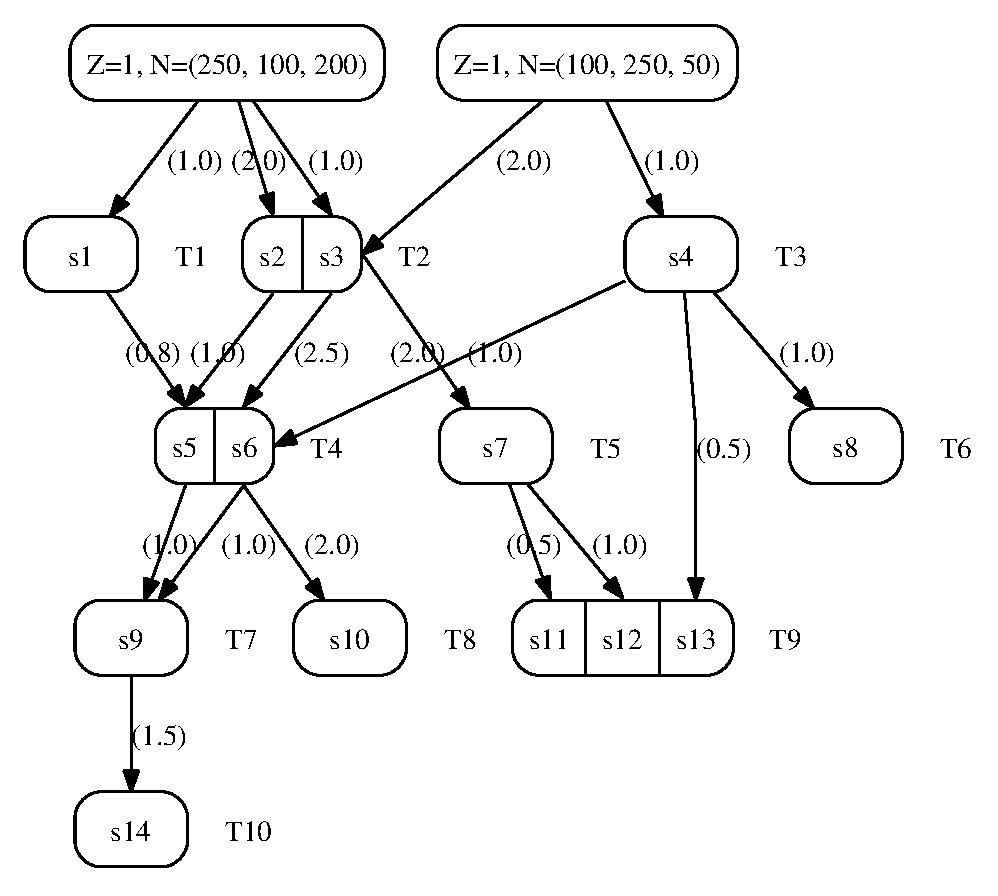
\includegraphics[scale=0.75]{image/example1services}
%\caption[An example small scale service center]{Represents an example small scale service center: the call graph of services and classes $y$, the  think times $Z$ and number of users $N$ of each class over time, the number of calls from classes to services and the invocation numbers within services $con$. }
%\label{fig:service_call_graph}
%\end{center}
%\end{figure}
%
%The class-to-service adjacency matrix obtained through the equations \ref{eq: compute-adjacency-matrix} from adjacency matrix of the service-class call graph is as follows: 
%\[
 %Y=\left(\begin{array}{cccccccccccccc} 1 & 2 & 1 & 0 & 2.8 & 2.5 & 1 & 0 & 5.3 & 5 & 0.5 & 1 & 0 & 7.95\\ 0 & 0 & 2 & 1 & 0 & 7 & 2 & 1 & 7 & 14 & 1 & 2 & 0.5 & 10.5 \end{array}\right)
%\]
%
%There are 6 available hosts to support the services. Capacity of the hosts are as  $\capp=[16\ 6\ 6\ 16\ 6\ 6]^T$ and their CPU speed factor is $\speedFactor=[1\ 1.2\ 0.9\ 1.1\ 0.8\ 1.2]$. The infrastructure cost coefficient was considered %roughly equal for all hosts except 
%a  random component that was added to break the symmetry and make the solution sparse: 
%$ \text{cost}=\text{rand}(H,T) $. 
%
%\newcounter{example}
%\addtocounter{example}{1}
  %\subsection{Example \arabic{example}: A Comparison of the Optimal Control and the Step-by-Step Optimization, a Hypothetical Case of a Fully Known Workload}      
 %In this simple example, we show the effect of solving a service placement problem through the optimal control framework. We show that if an objective is to avoid reconfiguration, and the workload has oscillations, the optimal control provides better results than the step-vise optimization.
 %
 %In order to make it simpler to understand, in this example, we make some unrealistic assumptions. We assume the service center has a very short lifetime of three time steps: $T=4$. The workload for this example was considered to be: 
%\[
%N=\left(\begin{array}{cccc} 0 & 220.0 & 150.0 & 200.0\\ 0 & 100.0 & 170.0 & 110.0 \end{array}\right)
%\]
  %Here, because of the limited number of timestamps, we need to make the assumption of fully knowing the workload for the whole simulation interval. In the next examples, however, we show for the optimal control approach to work, there is no need for knowledge or prediction of future workload.  The only assumptions is that at any given interval the workload has a  mean value.  % and this mean value tends to move slowly. 
   %
 %The response time SLA for all the steps were set to:  $R^\text{SLA}_t = [0.146 \  0.267]^T$. Based on the equation \ref{eq:convert-response-time-SLA-throughput} the optimizer substitutes $R_{SLA}$ and $N$ by:    
%\[
  %X_{SLA}=
%\left(\begin{array}{cccc} 0 & 192.0 & 130.9 & 174.5\\ 0 & 78.93 & 134.2 & 86.82 \end{array}\right) 
%\] 
%
 %The optimization was applied in two settings: with and without a relocation cost. Solving the overall optimization problem with a zero relocation cost, gives the same answer as solving a set of individual optimizations for separate steps.           
 %In other words, the optimizer acts in a fully reactive mode, doing its best to obey the SLA at each step.   
 %In the second case, the relocation cost is taken into account and the optimizer tries to satisfy the SLAs while minimizing the total number of relocations \footnote{In fact the controller tries to minimize the amount of resource adjustment to the services replicas, but this, in most cases means minimizing the number of replica relocations.  }. 
 %Also, note that in both cases the hosts are initially empty and no replica is deployed on them: $\theta_{s,h,0} = 0 \text{   for all $s$,$h$.}$. 
%
  %%  \subsubsection{Overall Optimization} 
 %In the overall optimization case, the optimizer achieves the desired throughput by an initial deployment of 19 service replicas in the first step and a total addition of 0 and removal of 0 in the subsequent steps (total changes of 19). 
%The placement at each step is demonstrated in Figure \ref{fig:overal_optimal_example}. It represents the placement decision at t=0. %
%%
%%
%\begin{figure}[htbp]\begin{center}\subfloat[Overall optimal
%example][Initial placement decision (decision at
%$t=1$)]{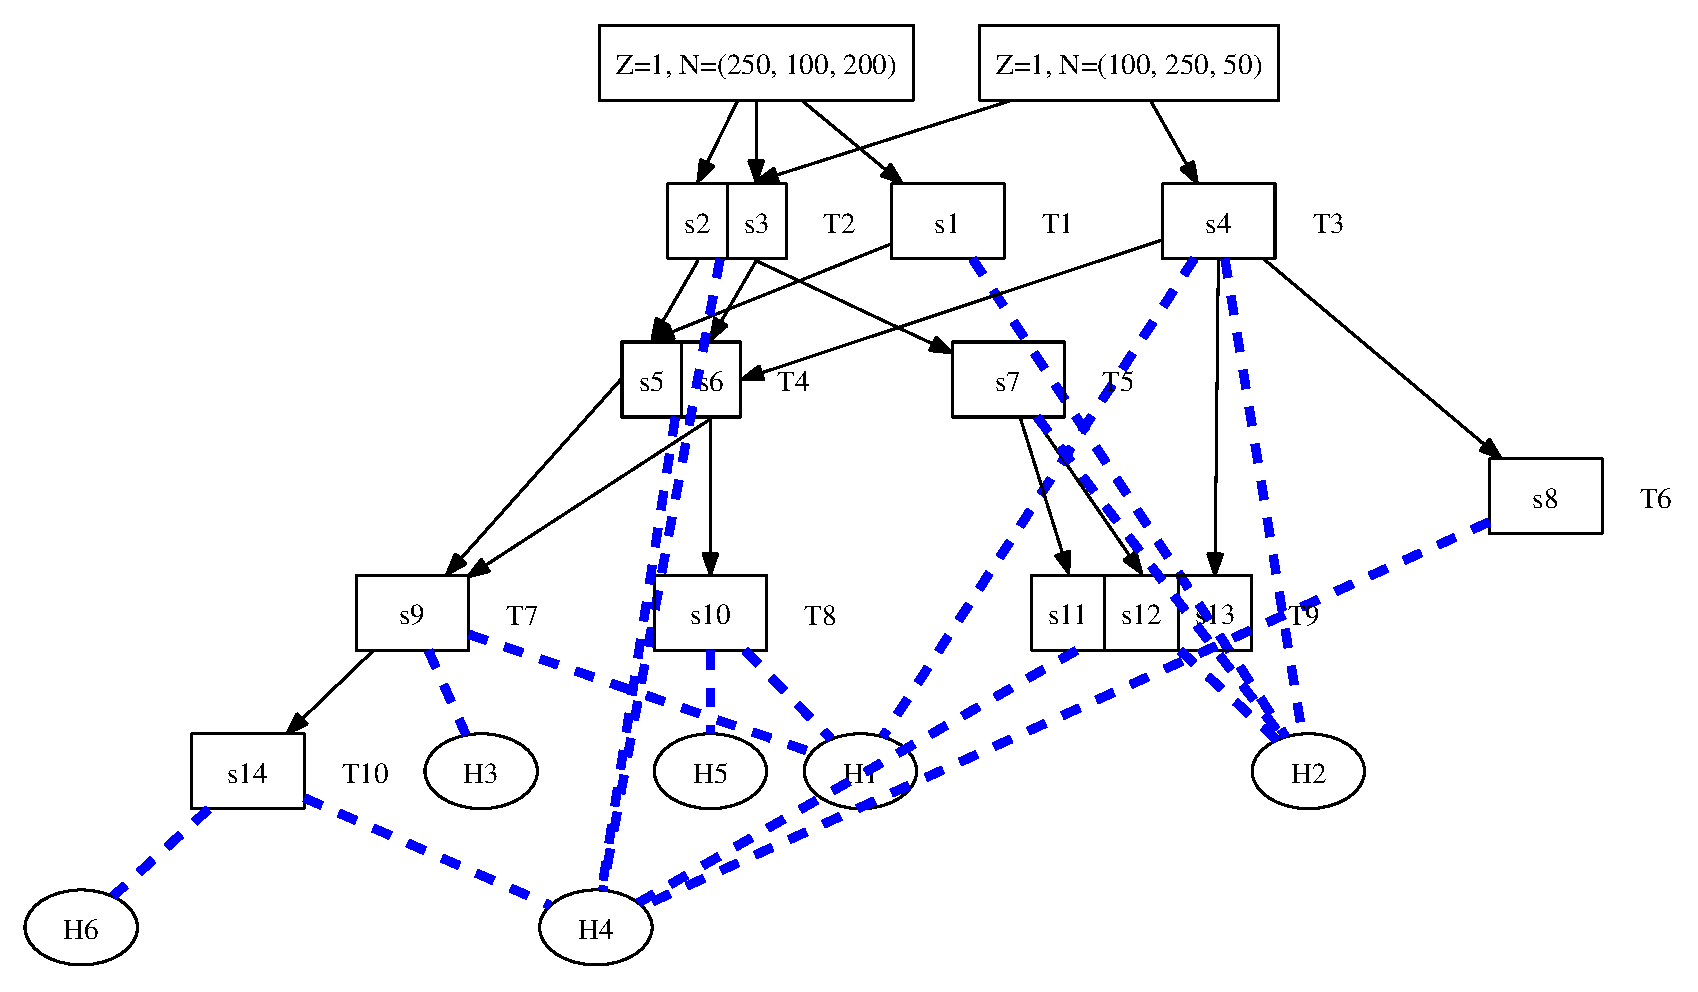
\includegraphics[scale=0.4]{image/example1deployment_overal_step1}
%\label{fig:subfig1}}
% [Represents the placement decisions for a small service center
%using the optimal control.]{Represents the placement decisions for a
%small service center using the optimal control.
%}\label{fig:overal_optimal_example}\end{center}\end{figure}%
%%
%% The (un)deployments are follows: 
%%
%%\begin{spacing}{1} 
%%
%%\begin{eqnarray*} 
%%
%%\begin{split}
%%
%%\text{t=2:} \\
%%
%%& 8   &  \text{added to }  & 2\\
%%
%%& 8  &   \text{added to } & 4 \\
%%
%%\text{t=3:}  \\
%%
%% &  3   &  \text{remove from } & 1 \\
%%
%%&   7  &    \text{added to } & 4 \\
%%
%% &   8  &    \text{remove from } & 4 \\
%%
%%\end{split}
%%
%%\end{eqnarray*}  
%%
%%\end{spacing}
%%
%%  
%%
%%
%%
%% At $t=2$ the container T8 is added to the hosts H2 and H4. this is because an increase in the class C2 population stresses the service $s10$. as  the workload of the second class decreases at $t=3$, containers T3 and T8 are removed from the hosts H1 and H4, and a replica of container T7 is added to the host H4. Note that the services on container T7 are mainly used by class C1. Also, see how service T8 is deployed on host H4 at $t=2$ but it is again removed from it in the next step,  $t=3$.
%%
%
 %% \subsubsection{Step-by-Step Optimization Ignoring the Relocation Cost}  
 %In the step-by-step optimization, where the relocation cost is ignored, the optimizer achieves the desired throughput by an initial deployment of 18 replicas in the first step and a total addition of 9 and removal of 11 in the subsequent steps (total changes of 38). The placements are depicted in Figure \ref{fig:stage_based_optimal_example}. 
%The undirected blue dashed lines denote the placements that have been added in the corresponding steps and the red dashed lines represent the placements that have been just removed at each time step. The black dashed lines denote the placements that performed in the past time step.
%
%\begin{figure}[htbp]
%\begin{center}
%\subfloat[Overall optimal example][Initial placement decision (decision at $t=1$)]{ \includegraphics[scale=0.35]{image/example1deployment_step1} \label{fig:subfig1}}  
 %\qquad  
%%
%\subfloat[Subfigure 1 list of figures text][Placement decision at $t=2$]{
 %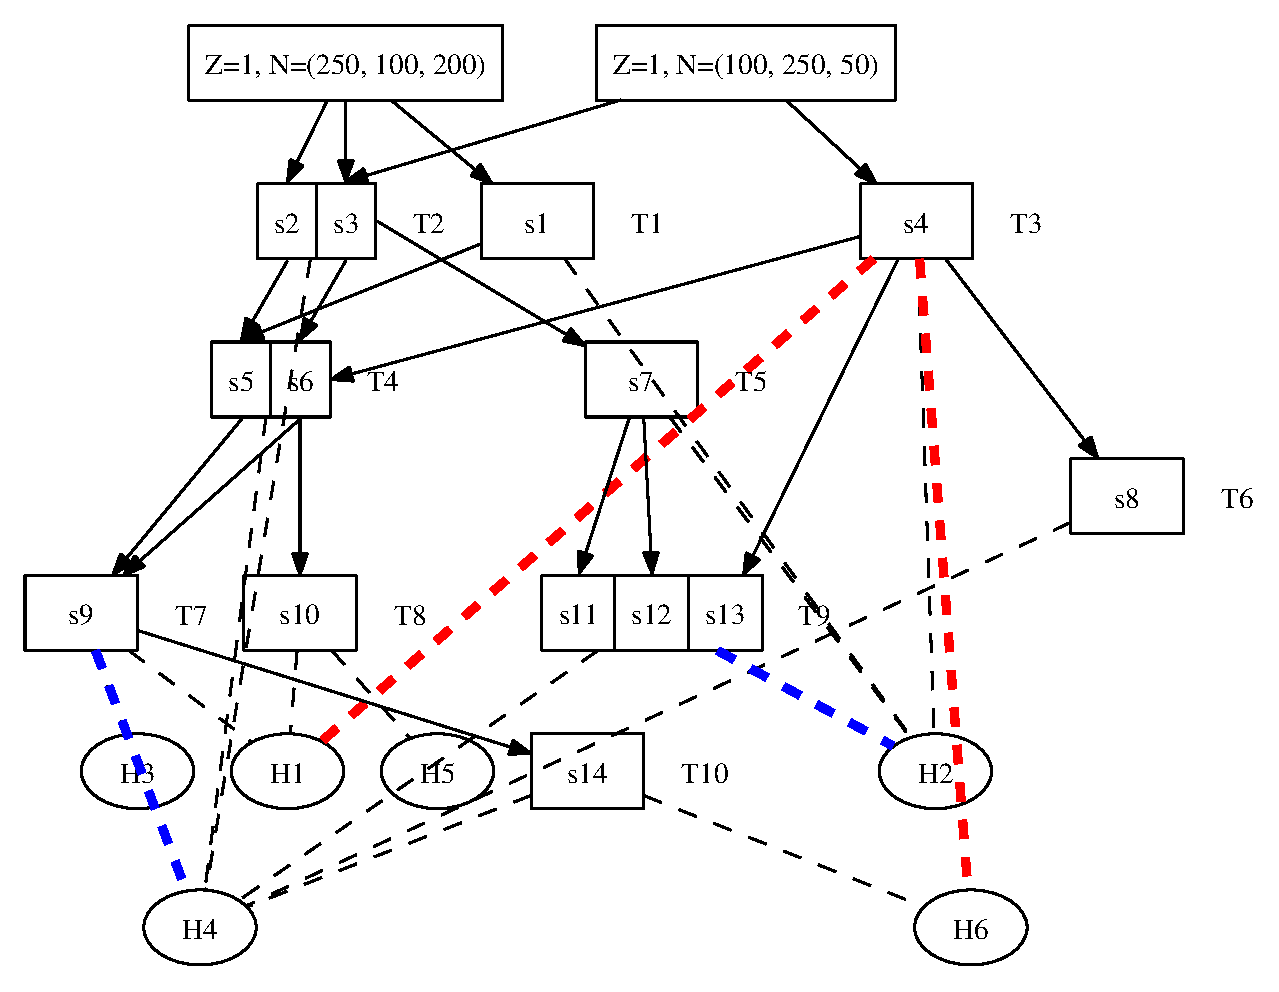
\includegraphics[scale=0.35]{image/example1deployment_step2} \label{fig:subfig2}} 
  %\qquad
%%
  %\subfloat[Subfigure 1 list of figures text][Placement decision at $t=3$]{
 %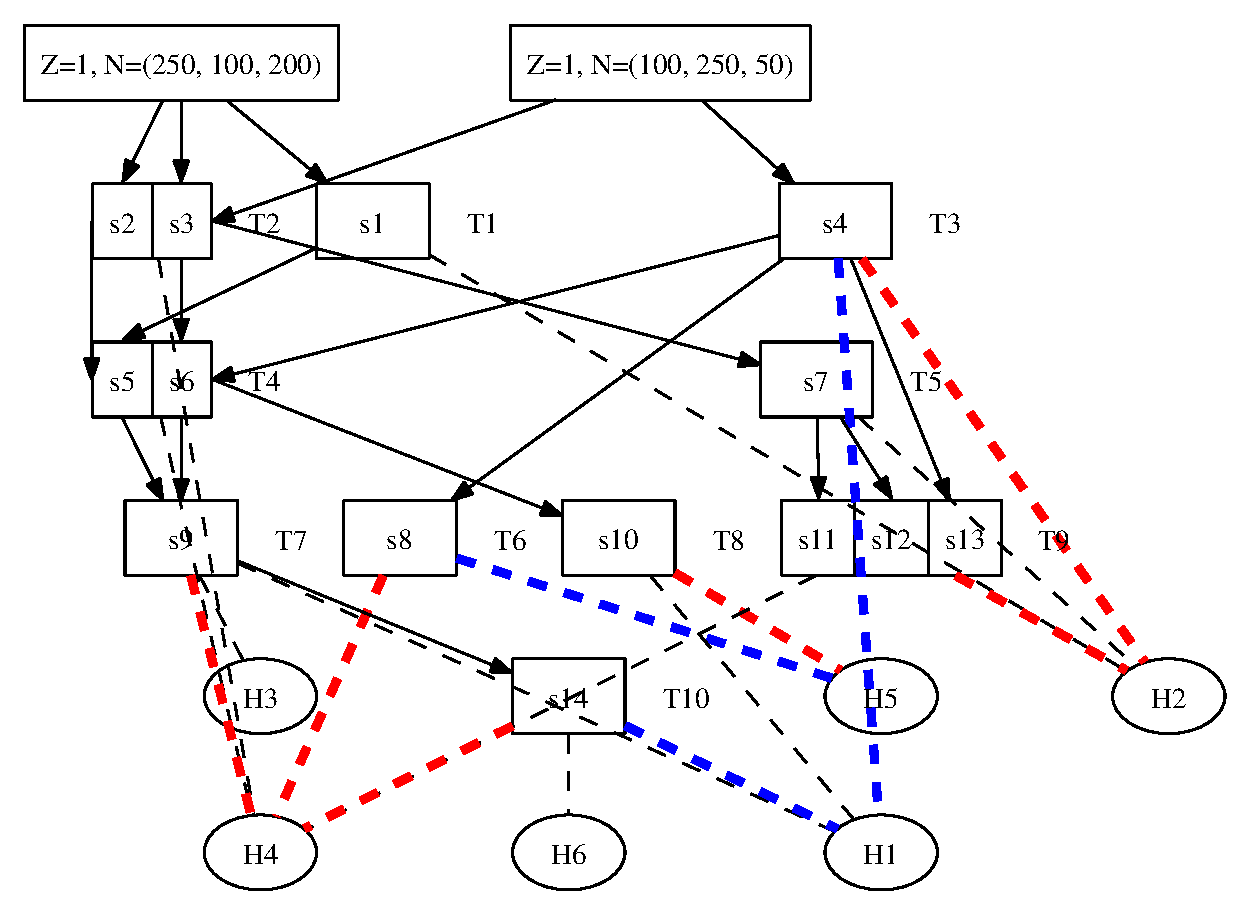
\includegraphics[scale=0.35]{image/example1deployment_step3} \label{fig:subfig3}} 
 %%
%\caption[An example of placement decisions for a small service center using step based optimization, ignoring the future steps.]{An example of placement decisions for a small service center using step based optimization, ignoring future steps.}
%\label{fig:stage_based_optimal_example}  
%\end{center}
%\end{figure}  
%
%and the (un)deployments are as follows:
%\begin{spacing}{1} 
%\begin{eqnarray*}
%\begin{split}
%\text{t=2:} \\
%& 4   &  \text{removed from }  &  4\\ 
%& 5   &  \text{removed from }  &  2\\ 
%& 5   &  \text{added to }  &  3\\ 
%& 9   &  \text{added to }  &  2\\ 
%& 10   &  \text{added to }  &  4\\ 
%& 14   &  \text{added to }  &  3\\ 
%& 14   &  \text{removed from }  &  6\\ 
%\text{t=3:} \\
%& 2   &  \text{removed from }  &  3\\ 
%& 2   &  \text{added to }  &  4\\ 
%& 4   &  \text{added to }  &  4\\ 
%& 4   &  \text{removed from }  &  5\\ 
%& 5   &  \text{added to }  &  2\\ 
%& 5   &  \text{removed from }  &  3\\ 
%& 8   &  \text{added to }  &  1\\ 
%& 8   &  \text{removed from }  &  5\\ 
%& 9   &  \text{removed from }  &  2\\ 
%& 10   &  \text{removed from }  &  4\\ 
%& 14   &  \text{removed from }  &  3\\ 
%& 14   &  \text{removed from }  &  5\\ 
%& 14   &  \text{added to }  &  6\\ 
%\end{split}
%\end{eqnarray*} 
%\end{spacing} 
%
%% note how services 6 and 10 are migrated in the same step.
 %These migrations increase the overall cost in the original objective function and make this solution suboptimal.
 %This clearly shows that when the cost of reconfiguration neglected,
%the overall optimality cannot be achieved in terms of original objectives (although optimization can be distributed over time steps). 
  %
%\addtocounter{example}{1}
 %\subsection{Example \arabic{example}: The Controller Reaction to Adding a Service} 
%In this example, we show how the controller responds to arrival of a new class of users. 
  %Consider the same small size service center.  In this example we assume that the system is already stabilized to the $N_{c1}=160$ users of class $c1$ with response time goal of $R^\text{SLA}_{c1}=0.146$. The class c2 joins the system at $t=1$ with a population of $N_{c2}=100$ and a SLA of $R^\text{SLA}_{c2}=1.146$. The controller uses a quadratic stage cost function for reconfiguration. We performed a simulation of $T=100$ steps that captures the behaviour of a controlled service center until it converges to a steady-state value.   
  %
 %Figure \ref{fig:adding_class_host_portion} represents the response of the system in terms of the utilization of the hosts. Since most of the services for the class $c2$ are hosted on hosts h1 and h2, we see an increase in their utilization. The decreasing utilization of h3 and h4 is due to the departure of the service replicas from them.  
 %Figure \ref{fig:adding_class_serv_portion} shows the amount of resource given to each service, which is increased for all of the services after the 2nd class is added to the system. 
 %Figure \ref{fig:adding_class_throughput} presents the throughput of the classes. 
  %As noted  it takes around 7 steps for the throughput of the class c2 to reach its SLA value. The duration of this convergence depends on the reconfiguration cost coefficient which has been set it to $r_3=100$.  
    %
%\begin{figure}
%\begin{center}
%\subfloat[Service addition scenario, response of the system in terms of utilization of the hosts.][Utilization of the hosts over time.]{
 %\includegraphics[scale=0.4]{image/placement/adding_class_host_portion} \label{fig:adding_class_host_portion}} 
%\subfloat[Service addition scenario, amount of resource given to each service][Amount of resource given to each service]{
 %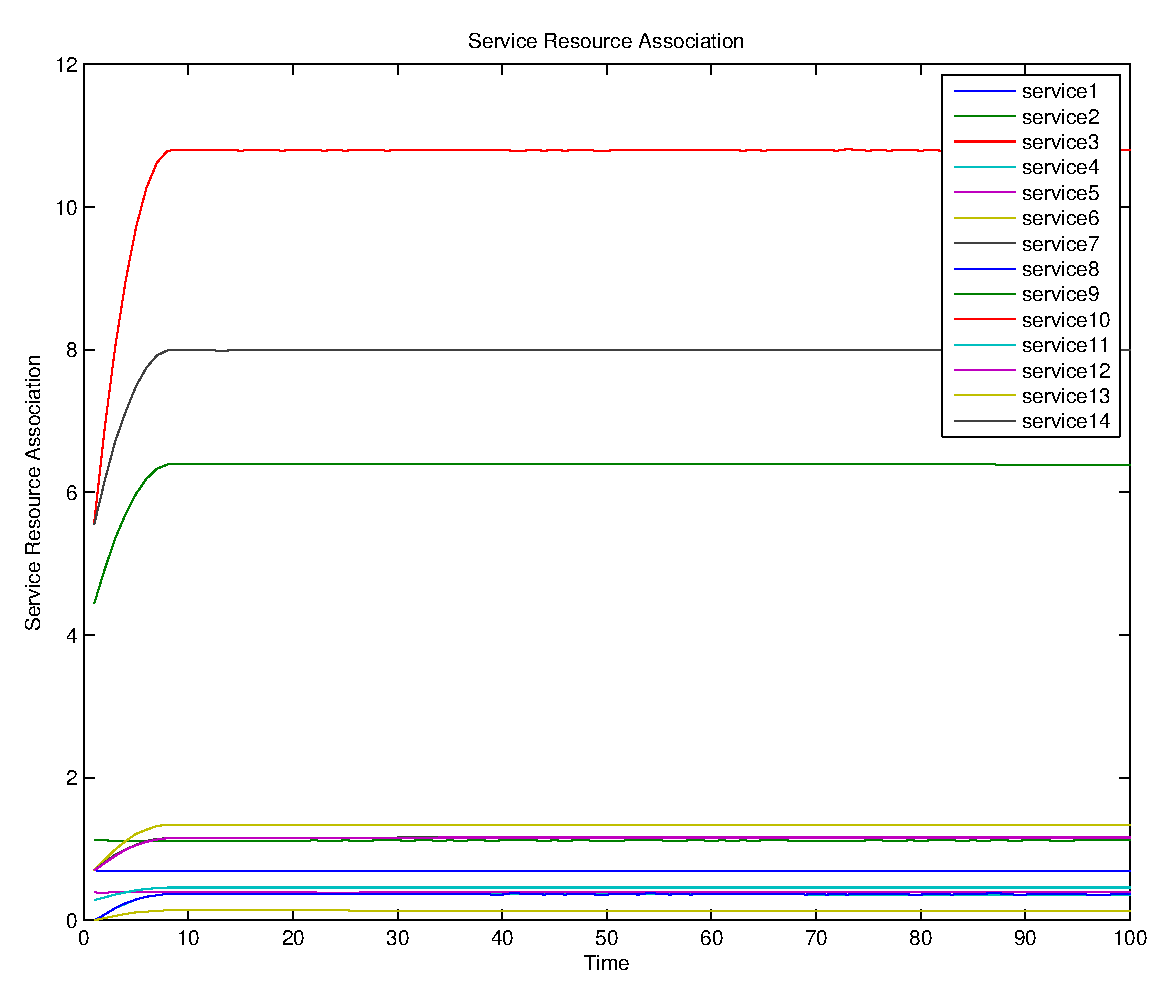
\includegraphics[scale=0.4]{image/placement/adding_class_serv_portion} \label{fig:adding_class_serv_portion}} 
  %\qquad
  %\subfloat[Service addition scenario, the throughput of classes][ the throughput of classes]{
 %\includegraphics[scale=0.4]{image/placement/adding_class_throughput} \label{fig:adding_class_throughput}} 
 %\subfloat[Service addition scenario, ][resource share of service replicas]{
 %\includegraphics[scale=0.35]{image/placement/adding_class_theta} \label{fig:adding_class_theta}}    
%\caption[Placement controller response to arrival  of a new class  of users]{Placement controller response to arrival  of a new class  of users. }
%\label{fig:stage_based_optimal_example}  
%\end{center}
%\end{figure}
      %Figure \ref{fig:adding_class_theta}    represents the service replicas whose resource share is affected more than 12\% of their original resource share.  Each square represents a  service replica at a certain time t.  The color intensity of the square represents the percentage of resource associated with the service  replica relative to its maximum during its lifetime. 
         %
      %\addtocounter{example}{1}
  %\subsection{Example \arabic{example}: Controller Reaction to Changing Cost Coefficient} 
   %In this example is shown how the distribution of service replicas can be changed using the change in placement coefficient, say from $c_1$ to $c_2$;  and how this transition is controlled by the controller over time in a way that it introduces minimal reconfiguration cost. A simulation is done over T=100 steps. 
  %
  %The workload and SLA of the system is assumed constant, $N=[160 100]'$, $Z=[1  1]'$, $RT_sla=[0.146  1.146 ]'$  during the experiment. 
   %The coefficients are assumed to be H-by-S matrix containing pseudorandom values drawn from the standard uniform distribution on the open interval (0,1) ($c_1=rand(H,S)$, $c_2=rand(H,S)$). 
 %The controller is initially assumed to have been driven by the workload, SLA, and placement coefficient $c_1$ and now in a stable state. 
  %At time $t=1$ the coefficient $c_2$ is suddenly  given to the controller to be applied.  
%\begin{figure} 
%\begin{center}
%\subfloat[Cost coefficient change scenario,  allocation of resources service replicas.][ Allocation of resources to service replicas. ]{\includegraphics[scale=0.35]{image/placement/test_change_cost_coef_theta_matrix} \label{fig:test_change_cost_coef_theta_matrix}} 
 %%
  %\subfloat[Cost coefficient change scenario, utilization of hosts.][Utilization of hosts.] {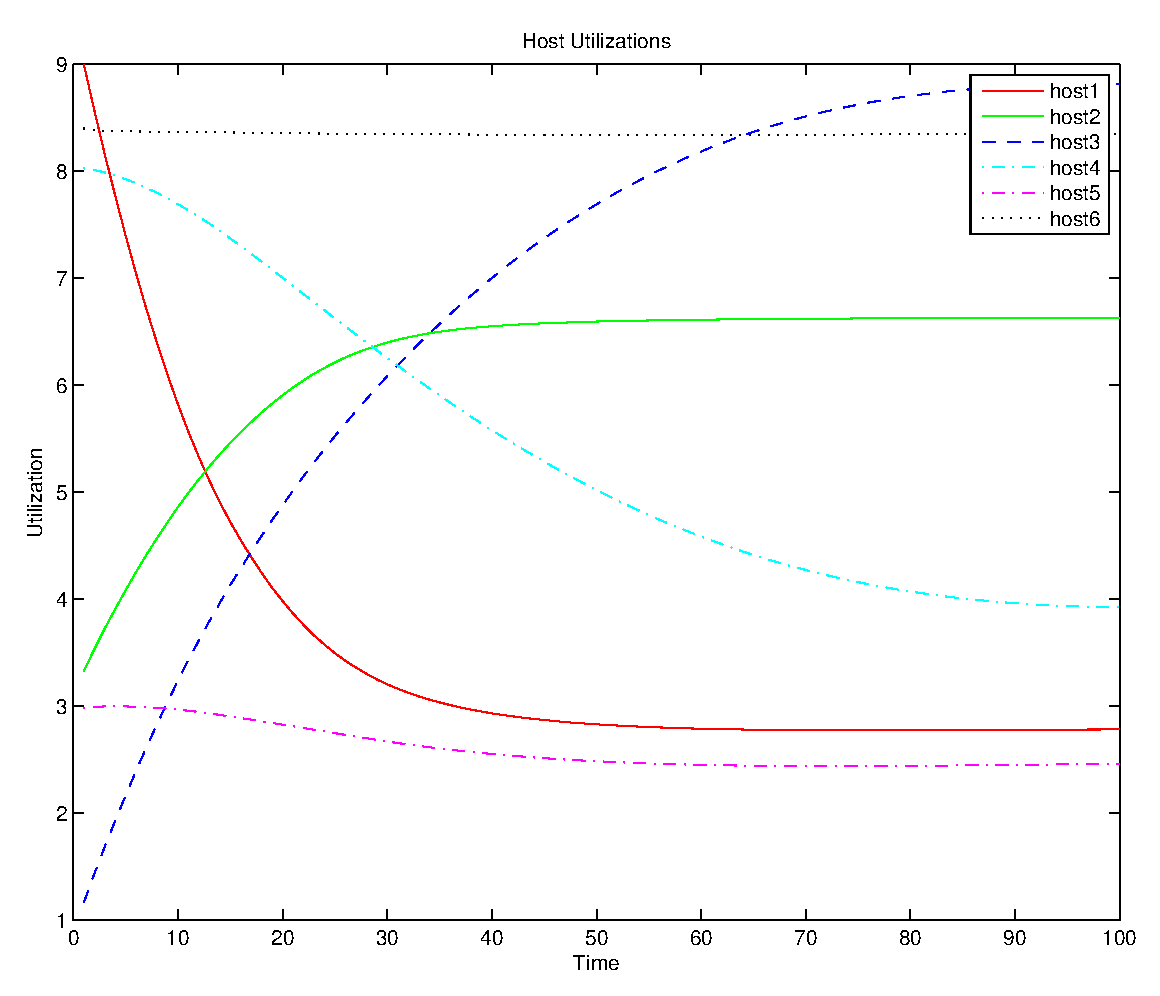
\includegraphics[scale=0.4]{image/placement/test_change_cost_coef_util} \label{fig:test_change_cost_coef_util}} 
%%
   %\qquad
  %\subfloat[Cost coefficient change scenario, stabilized placement at the beginning (red) and end (blue) of control interval. ][Stabilized placement at the beginning (red) and end (blue) of control interval.]{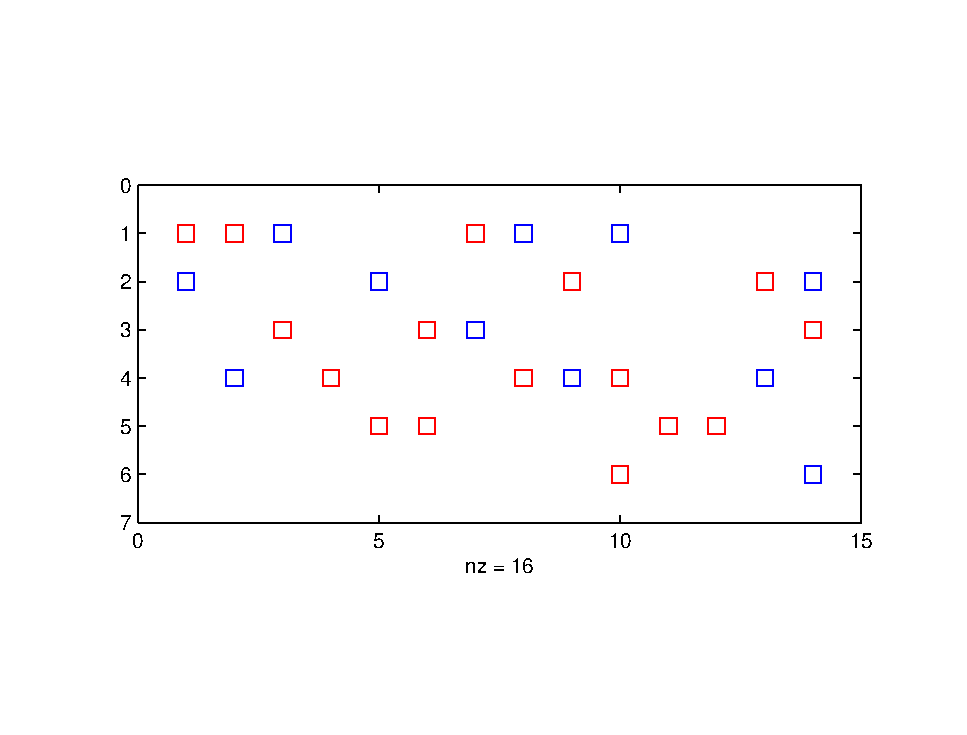
\includegraphics[scale=0.5]{image/placement/test_change_cost_coef_static} \label{fig:test_change_cost_coef_static}}   
  %%
   %\subfloat[Cost coefficient change scenario, service allocation of service replicas.][Service allocation of service replicas.]{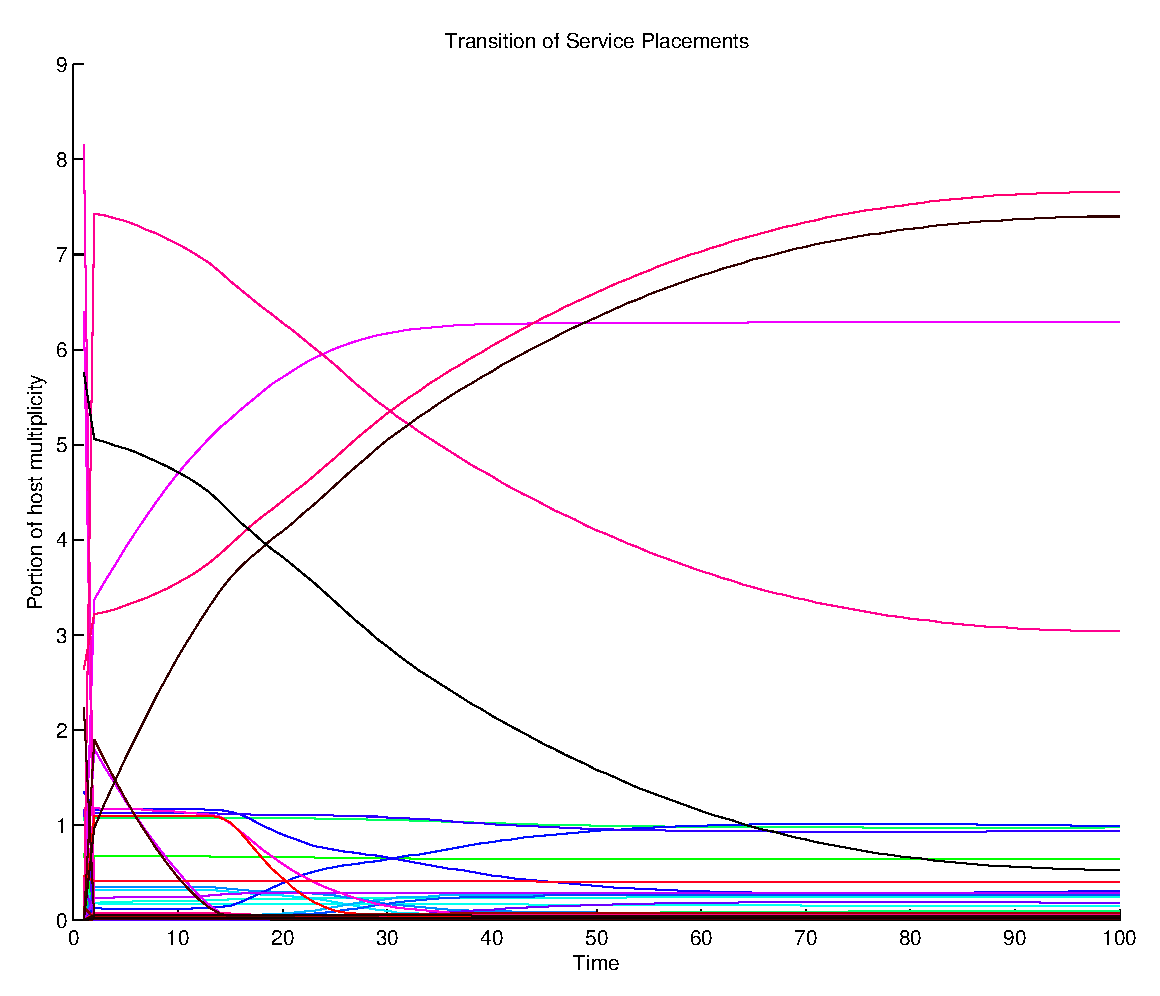
\includegraphics[scale=0.4]{image/placement/test_change_cost_coef_theta}    \label{fig:test_change_cost_coef_theta}}    
%\caption[Placement controller response to change in the cost coefficient.] {Placement controller response to change in the cost coefficient. } 
%\label{fig:cost-coefficient-change-scenario}  
%\end{center}
%\end{figure}
 %Figure \ref{fig:test_change_cost_coef_static}  represents the stabilized placement at the beginning  and end of control interval ( denoted by blue and  red markers  consecutively).  
  %Figure \ref{fig:test_change_cost_coef_theta}  represents the change of  allocated resource to service replicas during the control interval.  
   %Figure \ref{fig:test_change_cost_coef_util}  represents the utilization of the hosts over the control interval.  
%
 %\addtocounter{example}{1}
 %\subsection{Example \arabic{example}: The Controller Reaction to a Change in the SLAs }     
     %In this example, we show how the controller reacts to the changes in the response time SLAs. The workload and the optimization parameters, for the duration of this simulation, are constant and are as follows: $r=[5\ 1\ 100]$, $N=[160\ 100]^T$, $Z=[1\ 1]^T$, $c=rand(H,S)$. Between times $t=1$ and $t=100$ the response time SLA is as follows: $RT^\text{SLA}(t)=[0.46\  1.146 ]^T$. Between times $t=101$ and $t=200$ the response time SLA is as follows:  $RT^\text{SLA}(t)=[0.146\  1.146 ]^T$. The controller increases the amount of resource given to the service replicas in order to accommodate the more demanding SLA after t=100.   
    %
    %There is a small difference between this example  and the examples usually used in conventional  PID control;  instead of feeding the $RT^\text{SLA}(t)$ signal to the controller one step at a time, it is given to the controller in advance.  In other words we ask the controller to get the response time to the desired value at time step $T$. As a result,  using MPC becomes inevitable.  
  %\begin{figure}
%\begin{center}  
%\subfloat[The increase in the utilization of te hosts when the controller adjusts to a tighter SLA.][Increase in the utilization of the hosts when the controller adjusts to a tighter SLA.]{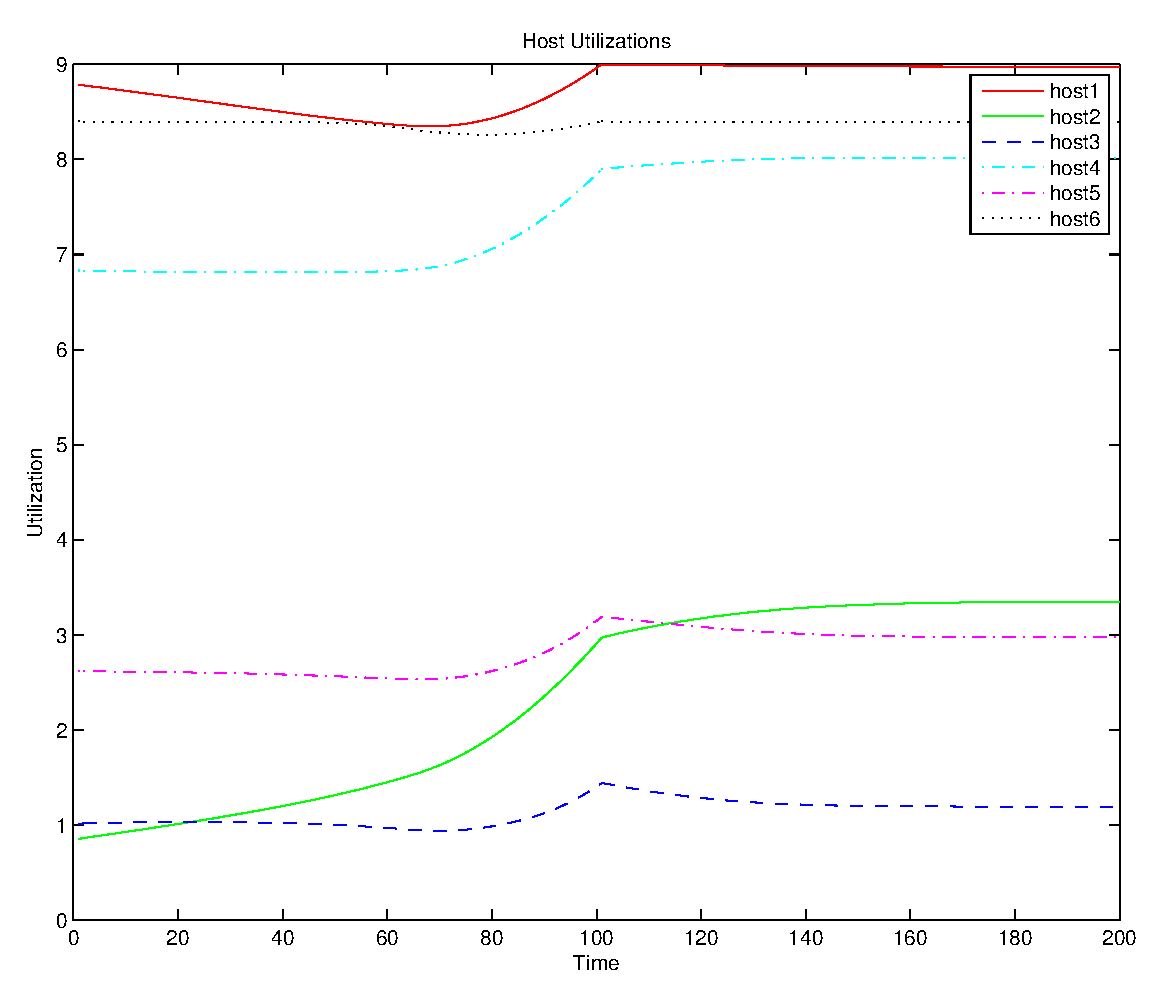
\includegraphics[scale=0.4]{image/placement/sla_change_host_portion} \label{fig:sla_change_host_portion}}
%%
%\subfloat[ Increase in the amount of resource  given to service replicas.][ Increase in the amount of resource  given to service replicas.]{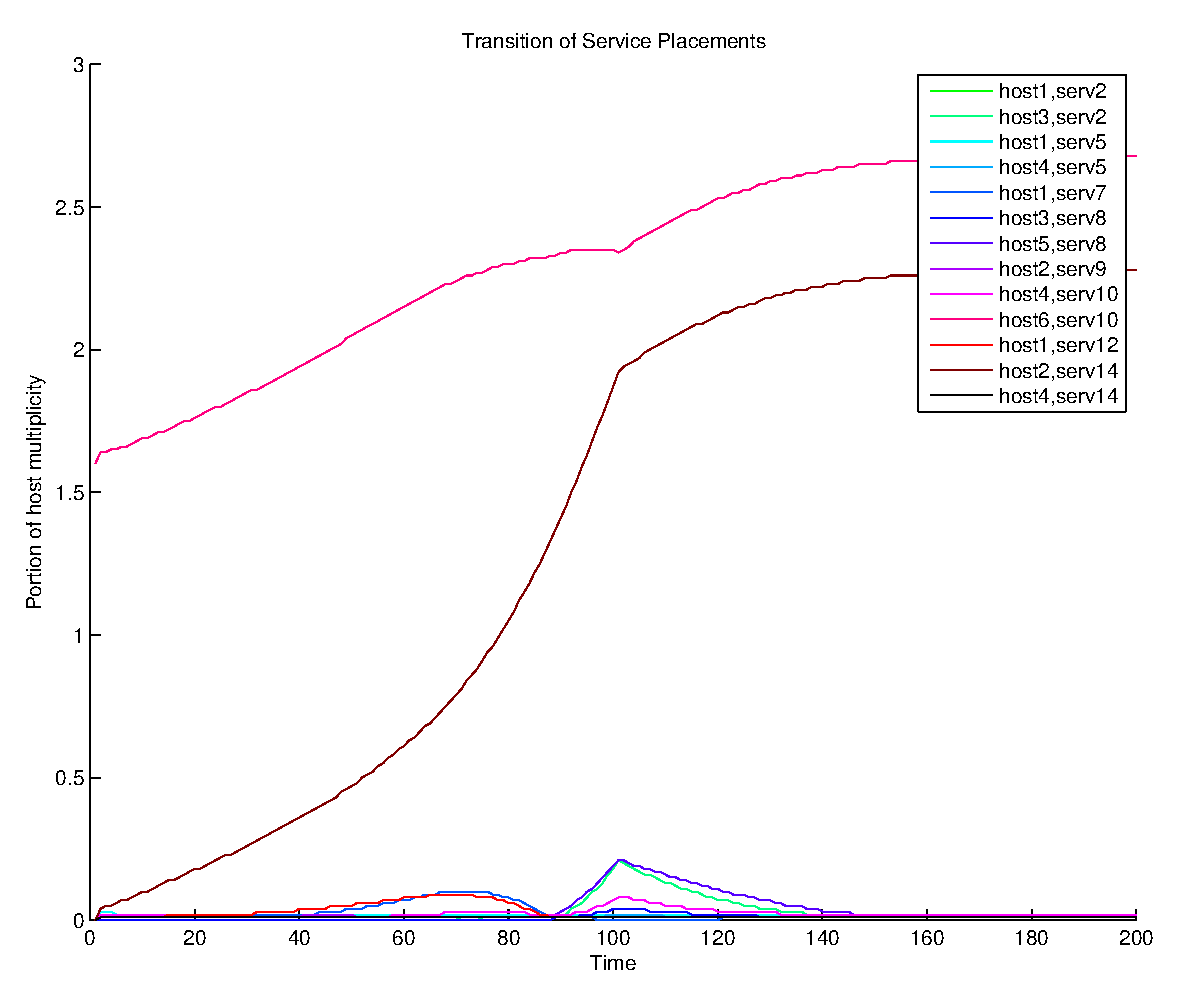
\includegraphics[scale=0.4]{image/placement/sla_change_theta}\label{fig:sla_change_theta}} 
  %\qquad
 %%   
%\subfloat[ Changes in the response time of class $c_1$ based on the given response time SLA.][Changes in the response time of class $c_1$ based on the given response time SLA.]{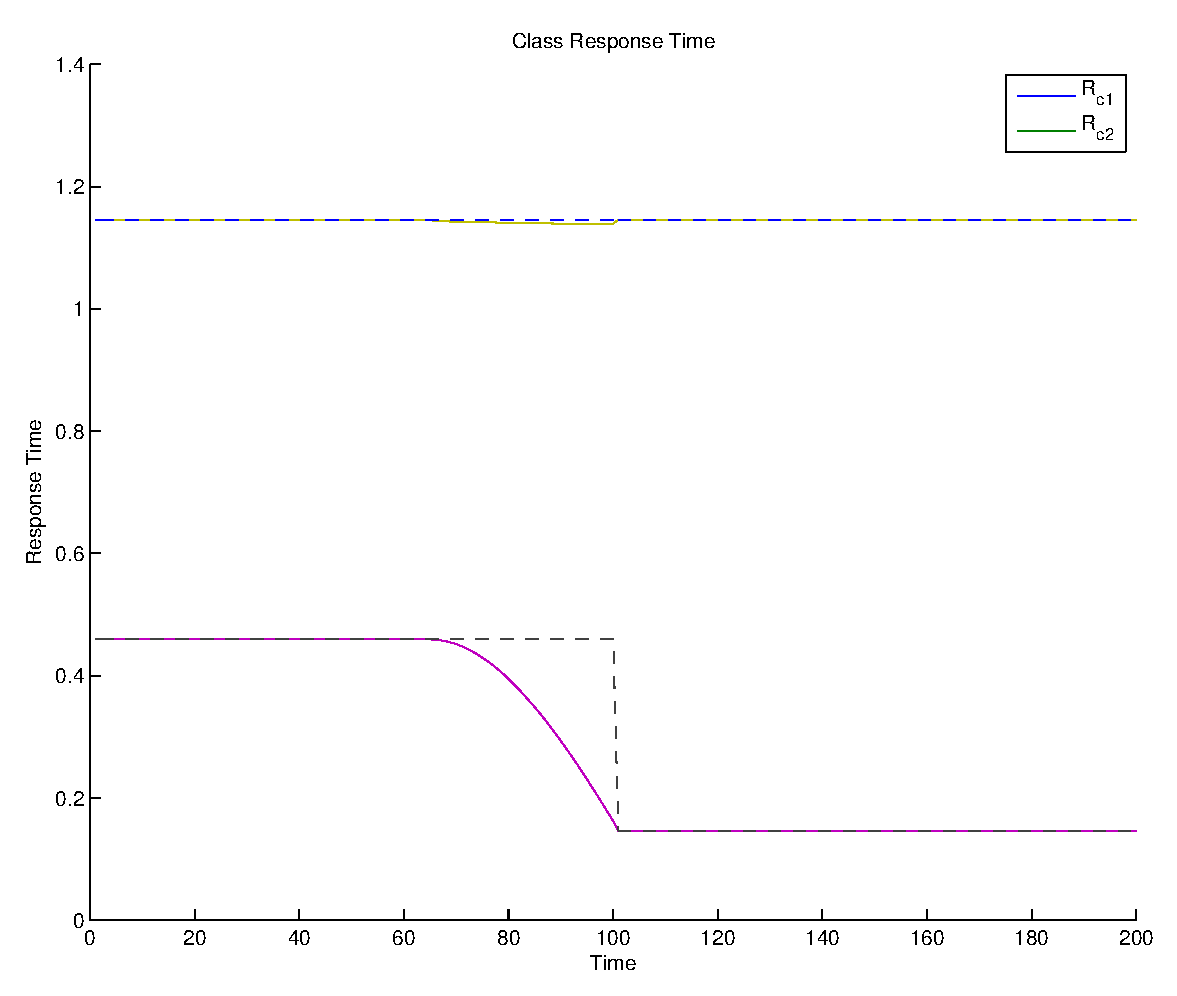
\includegraphics[scale=0.4]{image/placement/sla_change_rt} \label{fig:sla_change_rt} } 
  %\end{center}
%\end{figure}
%Figure \ref{fig:sla_change_theta}  shows how the services that are bottleneck are provisioned using more resources for their replicas in order to increase the throughput of the  associated class and improve its response time. Since services $s_{10}$ and $s_{14}$ are the major bottleneck for the class $c_1$ (whose response time SLA has decreased), the controller increases their portion of resources on hosts $h_6$ and $h_2$ respectively. 
     %Figure \ref{fig:sla_change_host_portion}  represents the change in the utilization of hosts when the controller adjusts to a tighter SLA. Figure \ref{fig:sla_change_rt} represents how the response time of class $c_1$ is driven to the specified SLA by a specified time.
    %
  %
 %\addtocounter{example}{1}         
 %\subsection{Example \arabic{example}: The Controller Response to a Dynamic Workload }   
   %In this example, we show how the controller reacts to a dynamic workload. 
 %Unlike the examples 1 to 6, that the input parameters to the system  (Workload, SLA, etc) change with a step like function pattern, in order to show the reaction of the controller, in this example we assume that the workload changes over time with a sinus like pattern. This is to investigate the response of the controller to a workload that introduces some thrashing.     
  %Figure \ref{fig:dynamic_workload} represents the workload.   
  %
   %In this example we set a relatively high cost coefficient value for the SLA violation cost ($r_\text{SLA}=50$  compared to $r_\text{resource}=1$). So the main trade-off is between the infrastructure and the reconfiguration costs.  
 %
  %\begin{figure}
%\begin{center}  
  %\subfloat[A sinus like workload][A sinus like workload] {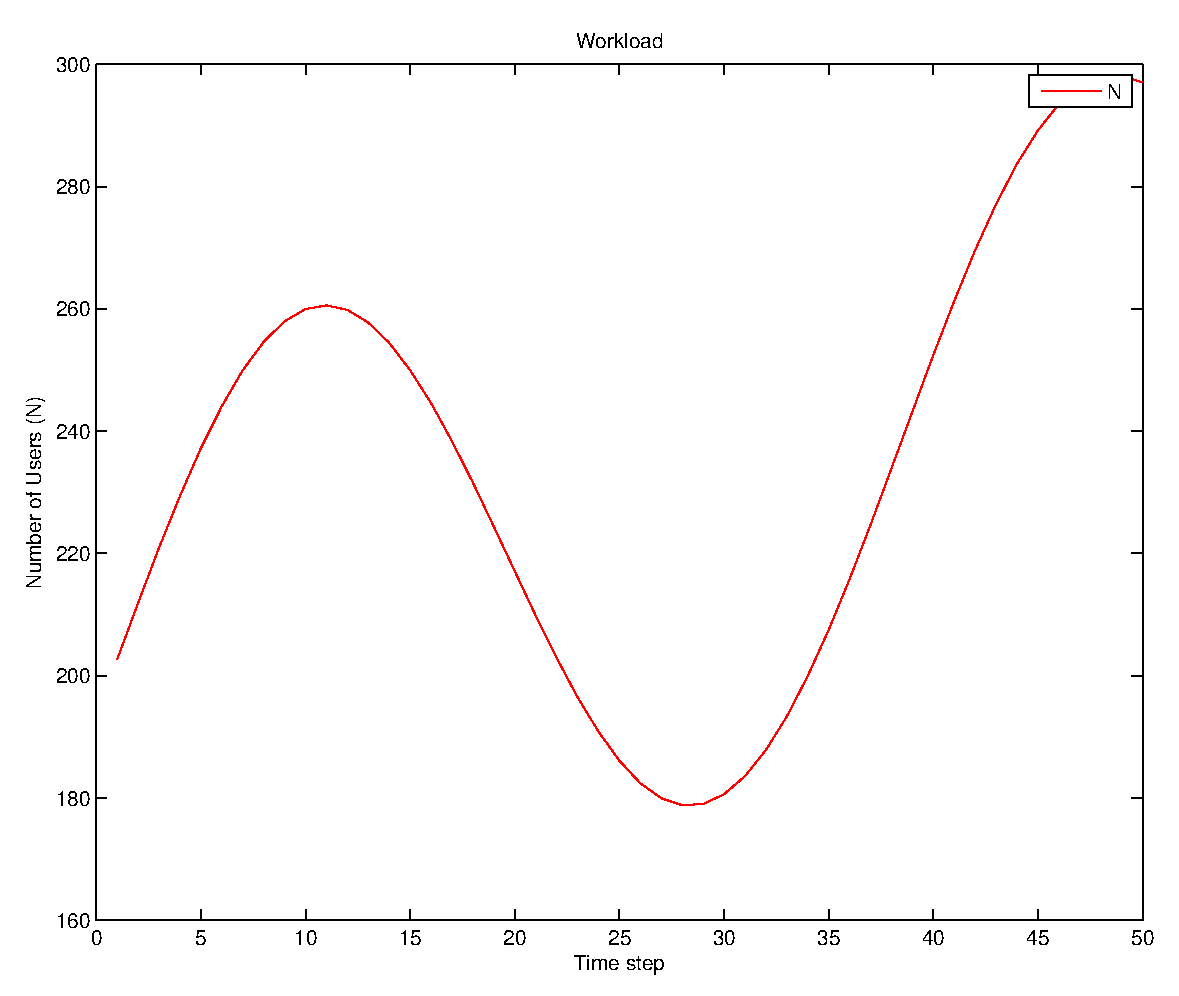
\includegraphics[scale=0.2]{image/placement/dynamic_workload.eps}\label{fig:dynamic_workload}  }  
  %\hspace{0.4cm}
  %%
%\subfloat[The cost of resource and the cost of reconfiguration for (optimal, MPC, no-reconfiguration-cost) placement controllers with parameters $T=7$ and $r_\text{trsh}=40$ and first norm reconfiguration cost function to a sinus like workload.][Resource cost and reconfiguration cost for the 1st norm penalty parameters $T=7$ and $r_\text{trsh}=40$.]{\includegraphics[scale=0.2]{image/placement/dynamic_infrastructure_cost_nsteps50_T7_rTRSH40abs.eps}
  %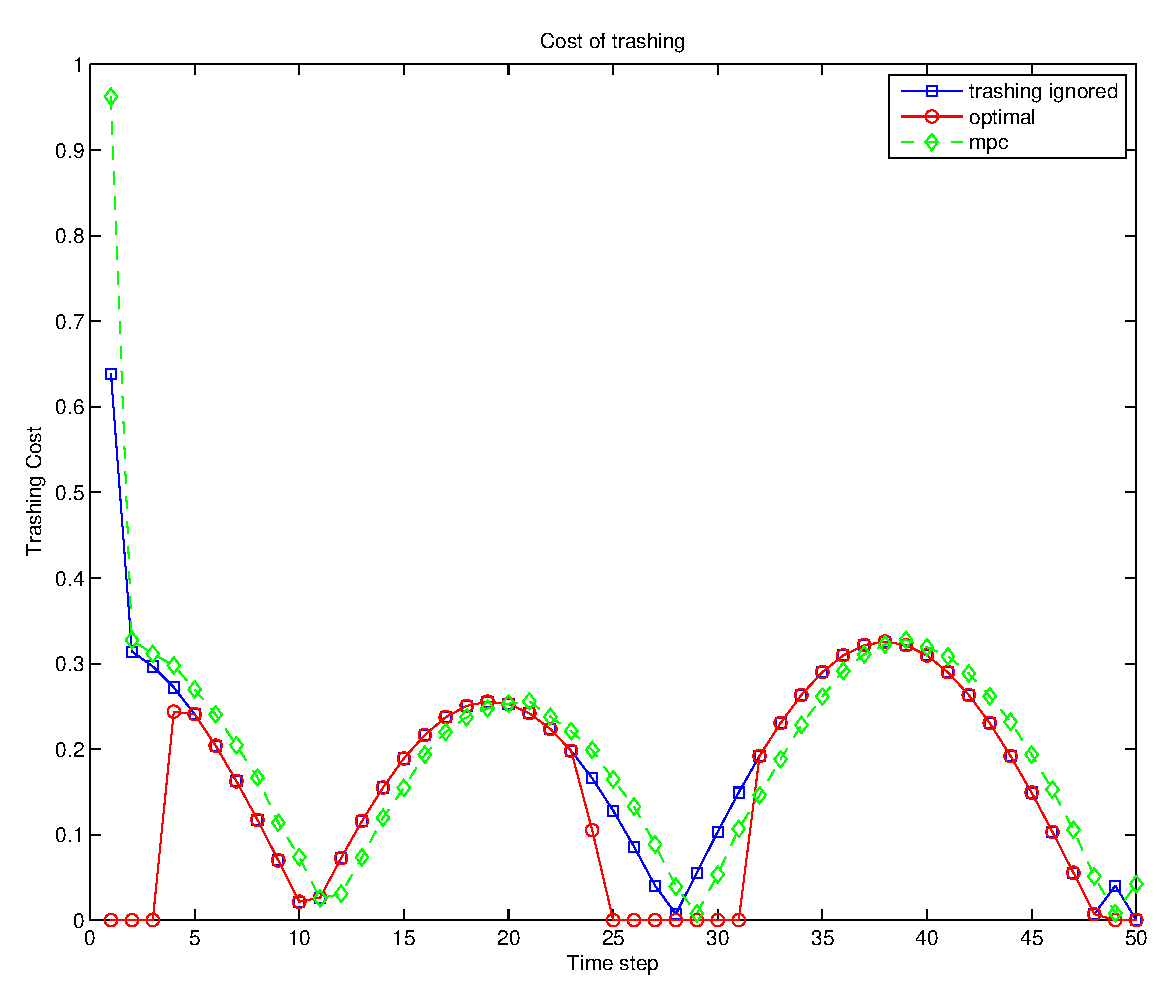
\includegraphics[scale=0.2]{image/placement/dynamic_trashing_cost_nsteps50_T7_rTRSH40abs.eps}
  %\label{fig:dynamic_cost_nsteps50_T7_rTRSH40abs}}  
 %\qquad
 %%
%\subfloat[The cost of resource  and cost of reconfiguration for (optimal, MPC, and no-reconfiguration-cost) placement controllers with parameters $T=7$ and $r_\text{trsh}=100$  and first norm  reconfiguration cost function to a sinus like workload.][Resource and reconfiguration cost for 1st norm penalty, and parameters $T=7$ and $r_\text{trsh}=100$.] {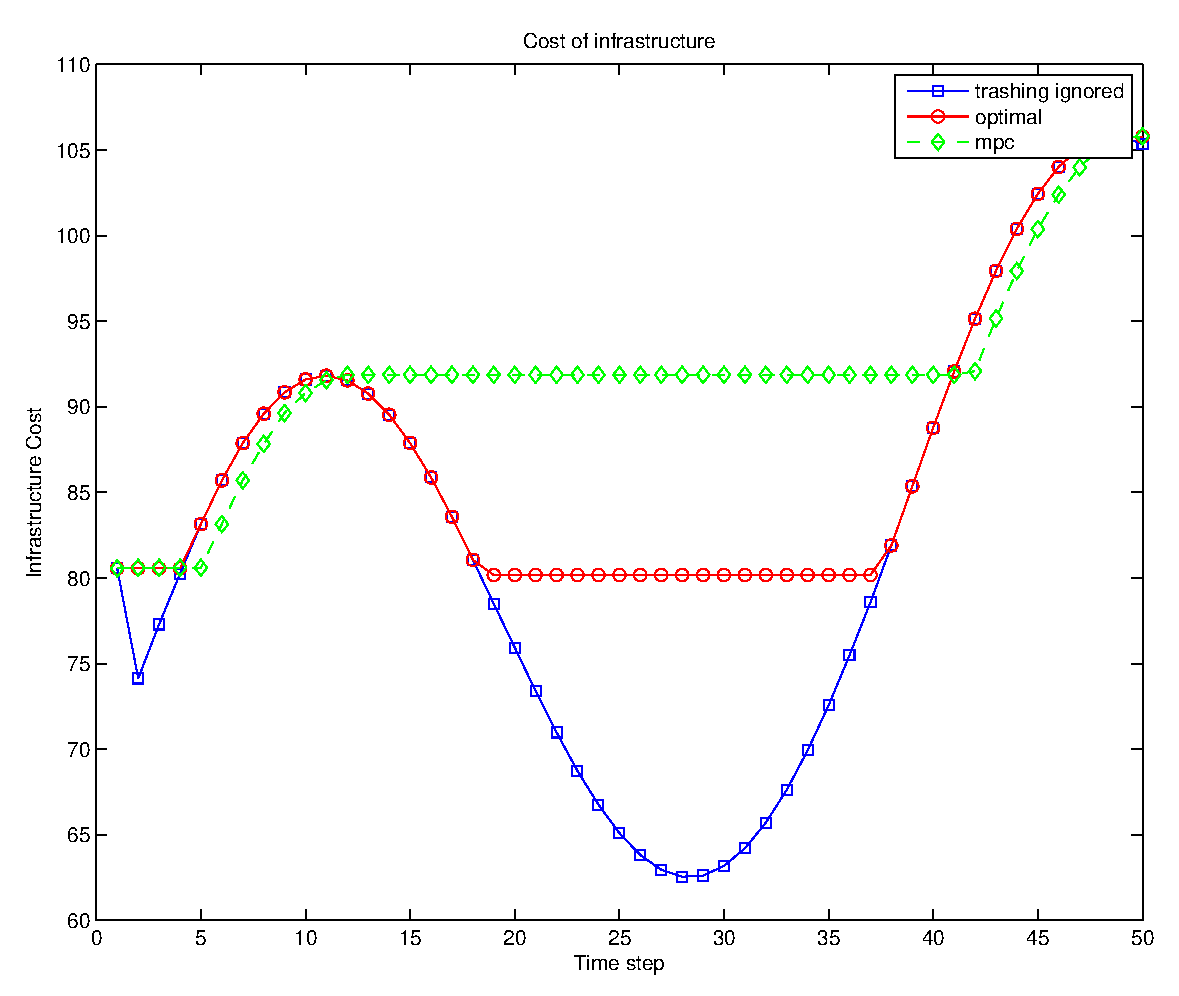
\includegraphics[scale=0.2]{image/placement/dynamic_infrastructure_cost_nsteps50_T7_rTRSH100abs.eps}
  %\includegraphics[scale=0.2]{image/placement/dynamic_trashing_cost_nsteps50_T7_rTRSH100abs.eps}
  %\label{fig:dynamic_cost_nsteps50_T7_rTRSH100abs}}   % \hspace{0.2cm}
  %%
 %\subfloat[The cost of resource  and cost of reconfiguration for (optimal, MPC, and zero-reconfiguration-cost) placement controllers  with parameters $T=7$ and $r_\text{trsh}=400$  and first norm  reconfiguration cost function to a sinus like workload][Resource and reconfiguration cost for 1st norm penalty, and parameters $T=7$ and $r_\text{trsh}=400$.] {\includegraphics[scale=0.2]{image/placement/dynamic_infrastructure_cost_nsteps50_T7_rTRSH400abs.eps}
%\includegraphics[scale=0.2]{image/placement/dynamic_trashing_cost_nsteps50_T7_rTRSH400abs.eps}
%\label{fig:dynamic_cost_nsteps50_T7_rTRSH400abs}}
%\qquad
%\subfloat[The cost of resource  and cost of reconfiguration for (optimal, MPC, and zero-reconfiguration-cost) placement controllers  with parameters $T=7$ and $r_\text{trsh}=400$  and second norm reconfiguration cost function  to a sinus like workload][Resource and reconfiguration cost for  2nd norm penalty, and parameters $T=7$ and $r_\text{trsh}=400$. ] {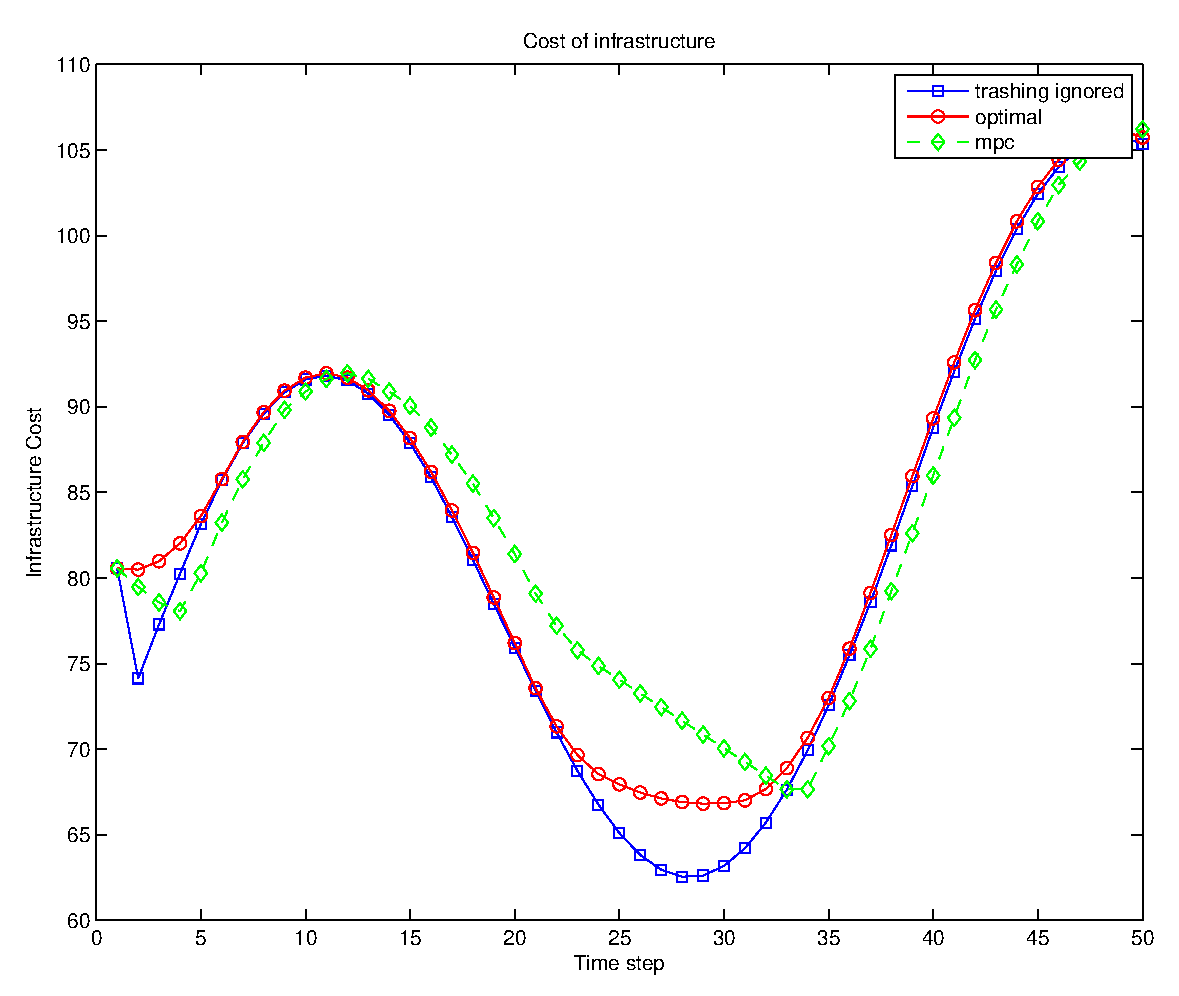
\includegraphics[scale=0.2]{image/placement/dynamic_infrastructure_cost_nsteps50_T7_rTRSH400square.eps}
%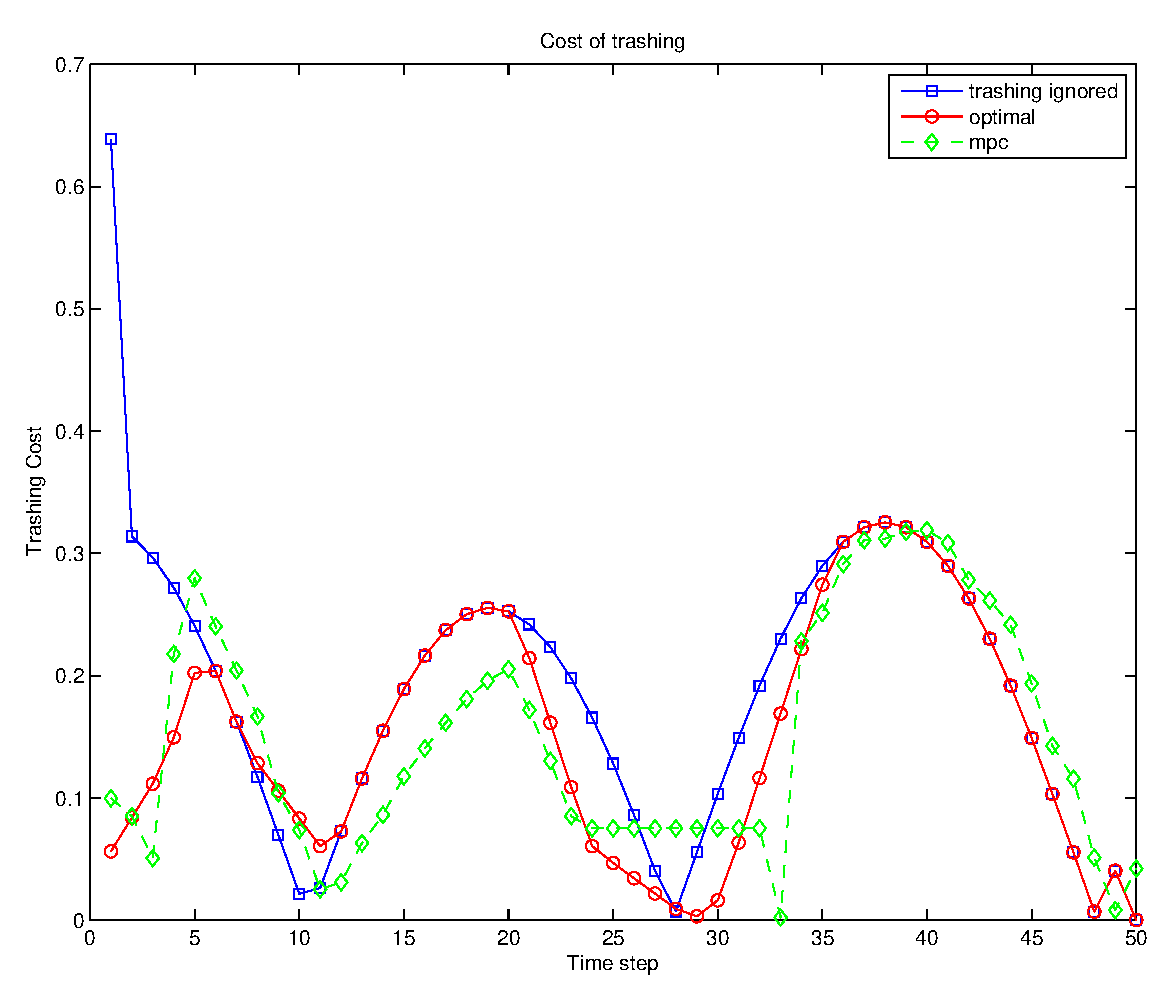
\includegraphics[scale=0.2]{image/placement/dynamic_trashing_cost_nsteps50_T7_rTRSH400square}
%\label{fig:dynamic_cost_nsteps50_T7_rTRSH400square}}  % \hspace{0.2cm}
%%
%\subfloat[The cost of resource  and cost of reconfiguration for (optimal, MPC, and zero-reconfiguration-cost) placement controllers  with parameters $T=7$ and $r_\text{trsh}=400$  and second norm reconfiguration cost function  to a sinus like workload. ][Resource and reconfiguration cost for 2nd norm penalty, and parameters $T=7$ and $r_\text{trsh}=4000$. ] {\includegraphics[scale=0.2]{image/placement/dynamic_infrastructure_cost_nsteps50_T7_rTRSH4000square.eps}
%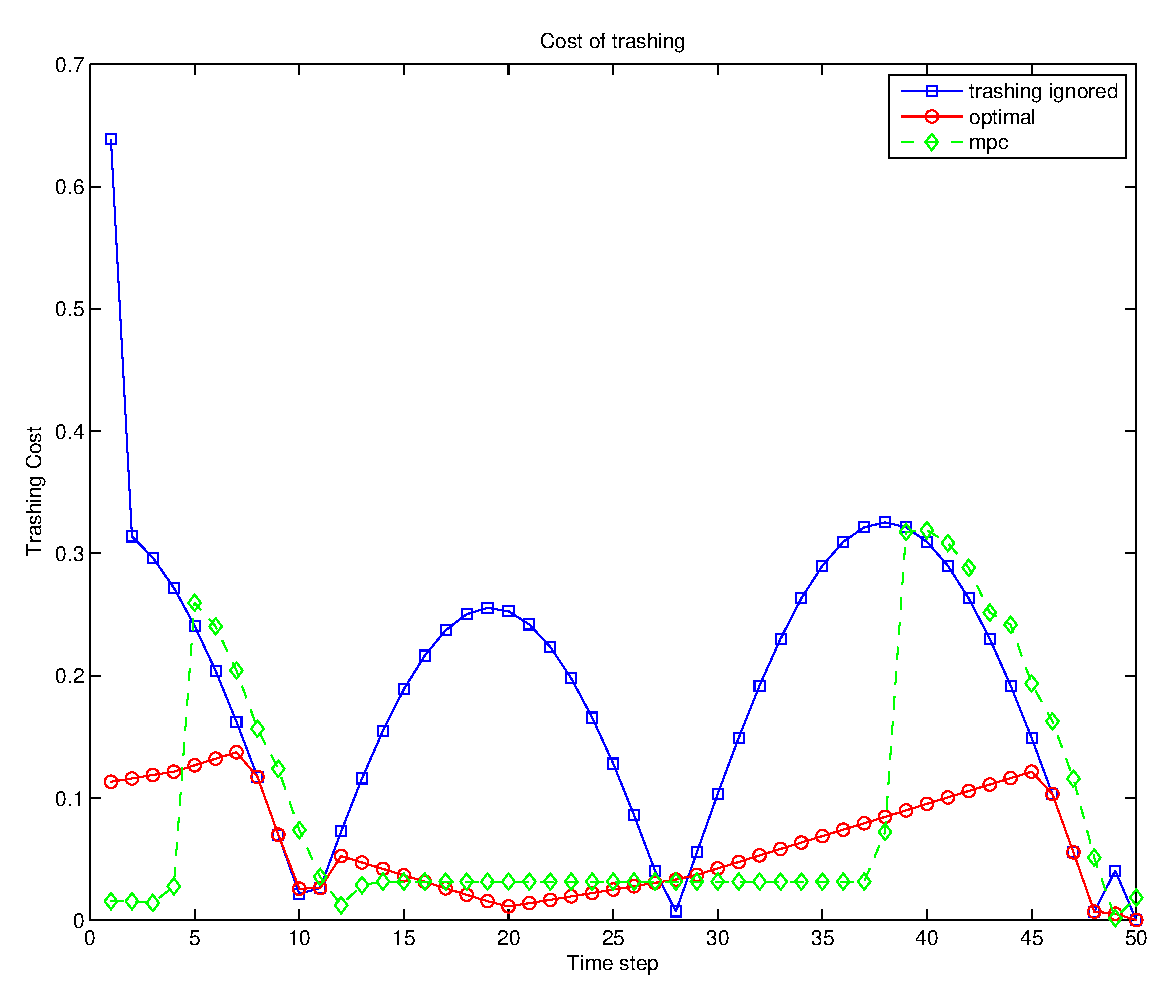
\includegraphics[scale=0.2]{image/placement/dynamic_trashing_cost_nsteps50_T7_rTRSH4000square}
%\label{fig:dynamic_cost_nsteps50_T7_rTRSH4000square}}
%%
%%
%\label{fig:cost-coefficient-change-scenario}  
%\end{center}
%\end{figure}
%
 %Figure \ref{fig:dynamic_cost_nsteps50_T7_rTRSH40abs} presents the cost of resource and the cost of reconfiguration for an optimal, MPC, no-reconfiguration-cost placement controllers when this workload is applied. The blue line in the figure represents the cost for the zero-reconfiguration-cost controller, a controller that has 0 reconfiguration cost coefficient and thus ignores the reconfiguration cost. The redline belongs to the optimal controller where it solves the optimal control problem for the whole interval assuming that the workload is known.  The green line represents the MPC controller. The MPC controller in this example uses the first norm function for the reconfiguration cost and has the parameter values of $T=7$ and $r_\text{trsh}=40$.  In figures \ref{fig:dynamic_cost_nsteps50_T7_rTRSH100abs} and 
   %\ref{fig:dynamic_cost_nsteps50_T7_rTRSH400abs}, we increase  the reconfiguration cost coefficient to 100 and 400 respectively. At $r_\text{trsh}=100$ we can see that the MPC controller completely gave up on adjusting to the decreasing workload but the optimal control still does some adjustment in response to the decrease.   
 %
 %When the reconfiguration's stage cost is defined using the first norm, the controller  `choice' between objectives becomes clear-cut. Unlike the second norm, where the controller compromises between the reconfiguration, preserving the SLAs, and infrastructure cost at every single timestep, a first norm stage cost controller makes  a clear decision on what objective to follow. As a result we see the controller is sometimes completely giving up the reconfiguration objective on workload ups and downs within the lookahead window (e.g. MPC controller in Figure \ref{fig:dynamic_cost_nsteps50_T7_rTRSH40abs}), sometimes giving up on saving infrastructure cost when workload decreases (Figure \ref{fig:dynamic_cost_nsteps50_T7_rTRSH100abs}), or the SLA violation cost when the workload increases. Essentially, with the first norm if the controller detects a change in the state of the system  (i.e. SLA, workload, or placement coefficients), it will either react to it immediately  or just ignores it.  
 %This decision is based on its prediction of change within the prediction window (e.g. $T=7$), and its behaviour depends heavily on this prediction. If the controller predicts that the change is permanent within the prediction window (i.e. it is not going to be reversed) then it might take immediate action based on the cost. If it detects that the change is temporary, then it most probably ignores doing a modification because of the reconfiguration cost. 
  %Its important however to note that detecting temporary changes in the time window using complicated models  is not necessary, because once the cycles of the workload are detected externally (i.e. by human administrator or a workload analyzer program)  the  cost coefficients and the prediction window of the controller can be updated to reach the desired behaviour  
 %\footnote{In order to change the costs for a specific classes  the cost coefficient scaler values  have to be substituted by vectors,  and there will be it a slight change in the objective function  to make  every  service have a different cost coefficient.}  
    %
  %Figures \ref{fig:dynamic_cost_nsteps50_T7_rTRSH400square} and  \ref{fig:dynamic_cost_nsteps50_T7_rTRSH4000square}  present the cost of resource  and cost of reconfiguration for different placement controllers  constructed with second norm reconfiguration cost function.
 %In \ref{fig:dynamic_cost_nsteps50_T7_rTRSH400square} the reconfiguration cost coefficient is set to $r_\text{trsh}=400$  while in \ref{fig:dynamic_cost_nsteps50_T7_rTRSH4000square}  it is $r_\text{trsh}=4000$.  In both cases and PC is suboptimal but it does a good job matching the optimal. 
%
%
%%   \begin{figure}
%%
%%\begin{center}
%%
%%\subfloat[Reaction of the  controller to the sinus like workload.][Reaction of the  controller to the sinus like workload.]
%%{\includegraphics[scale=0.4]{{image/placement/dynamictest_change_cost_coef_theta_matrix} \label{fig:test_change_cost_coef_theta_matrix}} 
%%   \qquad
%%
%%\end{center}
%%
%%\end{figure}
%%   
 %
%% \addtocounter{example}{1}
%% \subsection{Example \arabic{example}: Controller Response to Stochastic Workload}
  %
  %\section{Work That Remains}      
 %An example should be added in order to show the response of the controller to a stochastic workload. We are going to use two hours of FIFA98 workload to test the controller. A CEC implementation will be utilized where  
 %the mean of the workload parameters, calculated by moving average filters, are going to be used within the CEC controller. %for the whole lookahead window. 
%
  %One example should be added in order to assess the reaction of the controller to adding an unmanaged class.   In a real world, for example, this can be an administrative task run by administrators, or any other operating system process that consumes resources on the hosts. Services of this class are deployed together with managed services into the infrastructure.  The controller should react by moving replicas of the managed services, in a way that it keeps SLA of managed classes satisfied. 
  %% this should represent the response of the controller to addition of an unmanaged class; a class that there is no control over it's placement and resource allocation for its services. 
  %
 %
%% 
%
%%\addtocounter{example}{1}
%% \subsection{Example \arabic{example}: Controller Reaction to Adding an Unmanaged Service}    
%%   In this example we represent the response of the controller to addition of an unmanaged class. There is no control over the placement and resource allocation for services of this class.  In real world, for example, this can be an administrative task run by administrators, or any other operating system process that consumes resources on the hosts.  In terms of modeling, however, the class is modelled by its workload (whose Z, N, D are estimated) and ( hypothetical) services. Services are deployed together with managed services into the infrastructure.  The controller, thus, moves replicas of the managed services around to keep SLA of managed classes satisfied. 
%% 
 %
  %%  Example \arabic{example}:  Controller Response to Stochastic Workload  
  %
  
 \section{Case Study: The Controller Response to a Realistic Workload} 
 \label{sec:cases-study}  
  In this case study, we assess the reaction of the controller to a stochastic workload taken from a real application. The main objective is test the behaviour of the controller in terms of the ability to navigate the trade-off among SLA violations, resource cost, and the thrashing cost.  The structure of the services, the call graph, and the classes are the same as ones used in the motivating example (section~\ref{sec:motivating-examples}, Figure~\ref{fig:service_call_graph}).
   There are 14 services deployed on 6 hosts, possibly giving 84 service replicas. There are two classes of service utilizing the services.

	The workload for classes is a portion of the well-known FIFA98's workload obtained by processing the Web server logs. We processed the workload of the day 42 of FIFA98 to obtain the number of users for each five-minute interval. This gave 288 samples for the whole day (let us denote these by $N_t$).  We then constructed two 12 hour workloads for two class of users based on this as:
$N_{c1,t}=N_t-200$ for the first 12 hours and $N_{c2,t}= \lfloor N_{t+12h}/2\rfloor-110$ for the second 12 hours. These values are chosen so that the workloads of classes have peaks and valleys to test the controller. 
% Figure \ref{fig:dynamic_workload} presents the workloads in terms of the number of users $N_{c,t}$. 
The think times for the classes are $Z=[1, 1]^T$.
Multiplicity of hosts are $\capp=[9, 10, 10, 9, 10, 7]^T$.
The speed factors for the hosts are $=[1, 1.2, 0.9, 1.1, 0.8, 1.2]^T$
The service demand for the services are $d=[5, 4, 2, 8, 1, 2, 5, 8, 6, 8, 4, 5, 6, 5]\times 10^{-3}$.
The random cost coefficients are $\sigma^*_{s,h}=rand_{H,1}*\textbf{1}_{1,S}+10$.
 Each variable $rand_h$ is a value sampled from random variable of the uniform distribution, $U(0,1)$. 

 The system was simulated using the SimPy \cite{Mueller2003SimPy} simulator. The optimization problem was described using the \texttt{cvx} framework \cite{cvx} in Matlab where the problem is delegated to the SeDuMi \cite{sturm1999using} solver.  

 In this case study we performed two sets of experiments. In the first set we investigated the effect of different cost coefficients on the behaviour of the controller. In the second set of experiments, we investigate the effect of changing the length of lookahead horizon on the achievable cost trade-offs. 

\subsection{First Set of Experiments: Different Cost Coefficients}
We performed several experiments to test the response of the controller over time.
Here we show the detailed results for two simulations as representatives.
The lookahead horizon for MPC controller is five steps ($J=5$) for both experiments. 
	In the first simulation, we set the cost coefficients as follows: $[\rSLA=50,  \rResource=10, \rDeployment=4]$. 
In the second set, we set cost coefficients to: $[\rSLA=50,  \rResource=1, \rDeployment=40]$. Thus, intuitively the controller in the first configuration cares more about the cost of resources, while in the second configuration it cares more about the cost of reconfiguration. Let us call these controller configurations resource-precedent and reconfiguration-precedent controllers.
The result of simulations is depicted in figures \ref{fig:case_study_one_relocations}  
 to \ref{fig:case_study_one_response_time_cdf}.

 \begin{figure}[h]
\centering 
\subfloat[Resource Precedent Controller] {\includegraphics[width=0.5\linewidth]{image/placement/relocations_144steps_7T_50_10_4_abs}\label{fig:relocations_10_4}}
\subfloat[Reconfiguration Precedent Controller] {\includegraphics[width=0.5\linewidth]{image/placement/relocations_144steps_7T_50_1_40_abs}\label{fig:relocations_1_40}}
	\caption{The cumulative distribution function (CDF) of the number of relocations for two different MPC configurations.}
		\label{fig:case_study_one_relocations} 
\end{figure}
Figure \ref{fig:case_study_one_relocations}  represents the cumulative distribution function (CDF) of the number of relocations done for each time step for the resource-precedent controller (\ref{fig:relocations_10_4}) and the reconfiguration-precedent (\ref{fig:relocations_1_40}).
As can be noted, in Figure \ref{fig:relocations_10_4} the $Y$ value of the resource-precedent graph (red solid line) at 0 jumps to 0.6. This means 60\% of the area under the PDF curve is placed at 0. In other words, in 60\% of steps, there is no relocation. Compared to this, the CDF of the reconfiguration-precedent controller (blue dashed line) shows a lot fewer relocations per step; it has no relocation in almost 82\% of the steps.
%The rest of the steps have 1 to 20 relocations. 
%Only the first step has 70 relocations (not in the diagram), which is why the distribution is long tail. 

\begin{figure}[h]
\centering 
\subfloat[Resource Precedent Controller] {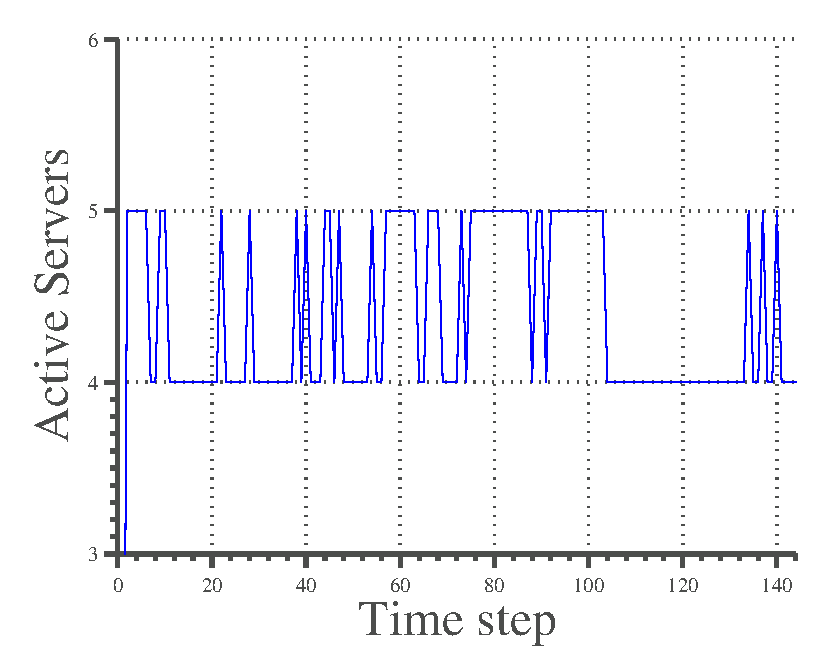
\includegraphics[width=0.5\linewidth]{image/placement/servers_144steps_7T_50_10_4_abs}\label{fig:servers_10_4}}
\subfloat[Reconfiguration Precedent Controller] {\includegraphics[width=0.5\linewidth]{image/placement/servers_144steps_7T_50_1_40_abs}\label{fig:servers_1_40}}
		\caption{The number of active servers over time for two different MPC configurations.}
		\label{fig:case_study_one_number_of_servers}  
\end{figure}
Figure \ref{fig:case_study_one_number_of_servers} represents the number of active servers over time in both configurations.
The figure is consistent with our assumption: the resource-precedent controller (\ref{fig:servers_10_4}) tries to save resources by deactivating/activating physical machines more frequently than the reconfiguration-precedent one (\ref{fig:servers_1_40}).


% has more oscillations. This is because more weight is assigned to the resource costs and less weight to reconfiguration cost; thus, 
%
\begin{figure}
\centering 
\subfloat[Resource Precedent Controller] {\includegraphics[width=0.5\linewidth]{image/placement/rt1_144steps_7T_50_10_4_abs}\label{fig:rt_10_4}}
\subfloat[Reconfiguration Precedent Controller] {\includegraphics[width=0.5\linewidth]{image/placement/rt_144steps_7T_50_1_40_abs}\label{fig:rt_1_40}}
	\caption{The raw response time graphs over time for two different MPC configurations.}
		\label{fig:case_study_one_response_time}
\end{figure}

 To show the extent to which the SLA is satisfied in each scenario, we have provided the raw response time graphs in Figures \ref{fig:rt_10_4} and \ref{fig:rt_1_40}.
\begin{figure}
\subfloat[Resource Precedent Controller] {\includegraphics[width=0.5\linewidth]{image/placement/rtcdf_144steps_7T_50_10_4_abs1}\label{fig:rtcdf_10_4}}
% \subfloat[] {\includegraphics[width=0.5\linewidth]{image/placement/rtcdf_144steps_7T_50_10_4_abs}\label{fig:ts1a}}
\subfloat[Reconfiguration Precedent Controller] {\includegraphics[width=0.5\linewidth]{image/placement/rtcdf_144steps_7T_50_1_40_abs}\label{fig:rtcdf_1_40}}
		\caption{The difference between response time and the response time SLA as a CDF for two different MPC configurations.}
	\label{fig:case_study_one_response_time_cdf}
\end{figure}
 However, it is not very easy to see their difference. In Figures~\ref{fig:rtcdf_10_4} and~\ref{fig:rtcdf_1_40} we represent the difference between the response time and the response time SLA (i.e. $RT_c - RT_c^\text{SLA}$) as a CDF, taking each time step as one sample. 
 %As can be observed, in both scenarios there is no shortage of throughput from the one specified in the SLA.
 In \ref{fig:rtcdf_10_4}, there were some points where the SLA is breached, and that is why the CDF increases into the region $RT_{c}>RT^\text{SLA}_c$. In \ref{fig:rtcdf_1_40}, the response time did not breach the SLA, and the CDF reaches 1 before the region $RT_{c}>RT^\text{SLA}_c$. 

%
%
%\begin{figure}
%\centering 
%\subfloat[] {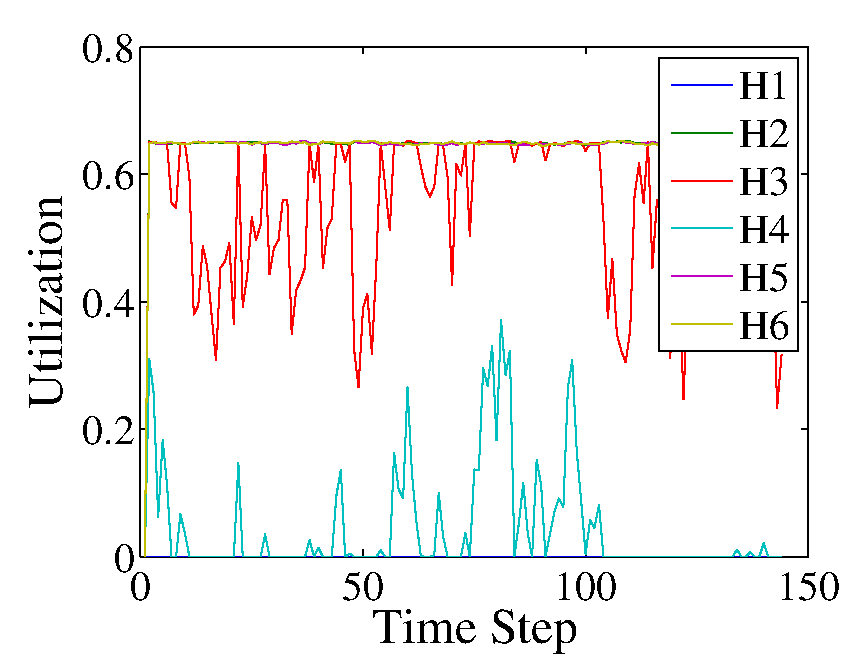
\includegraphics[width=0.5\linewidth]{image/placement/util_144steps_7T_50_10_4_abs}\label{fig:ts2a}}
%\subfloat[] {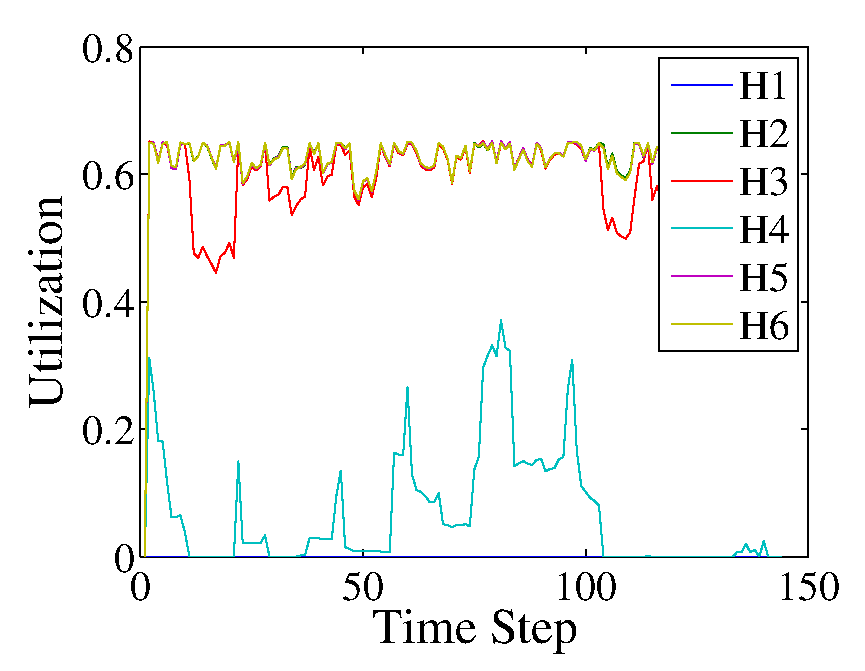
\includegraphics[width=0.5\linewidth]{image/placement/util_144steps_7T_50_1_40_abs}\label{fig:ts2b}}
	%\label{fig:case_study_one_utilization}  
	%\caption{what's up}
%\end{figure}




%\subfloat[] {\includegraphics[width=0.5\linewidth]{image/placement/relocations_144steps_7T_50_1_4_abs}\label{fig:ts1a}}
%\subfloat[] {\includegraphics[width=0.5\linewidth]{image/placement/relocations_144steps_4T_50_1_4_abs}\label{fig:ts1a}}
%\subfloat[] {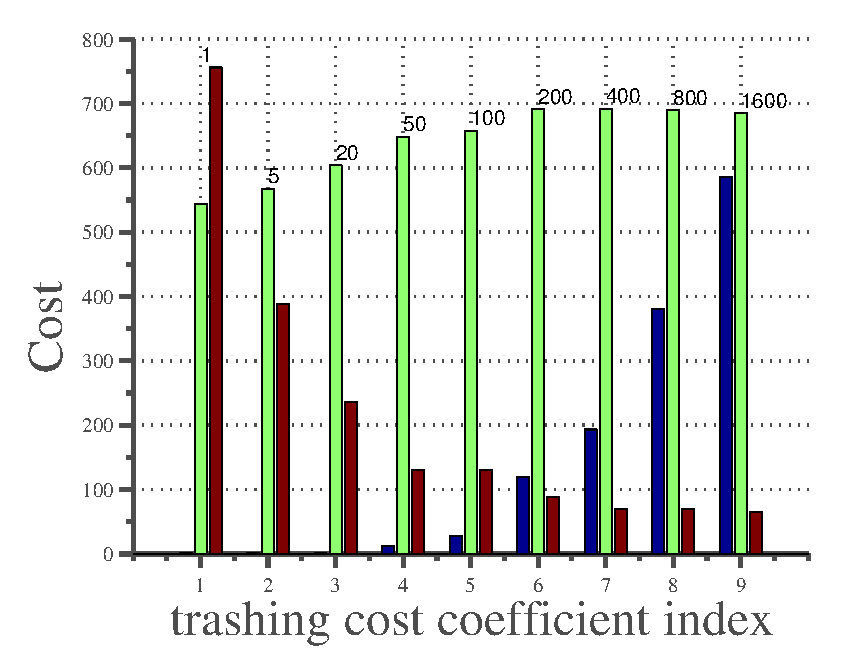
\includegraphics[width=0.5\linewidth]{image/placement/trade_off_50_1_abs}\label{fig:ts1a}}
%
	  %\subfloat[] {\includegraphics[width=0.5\linewidth]{image/placement/relocations_CDF_compare}\label{fig:ts1a}}
	  %\subfloat[] {\includegraphics[width=0.5\linewidth]{image/placement/active_servers_CDF_compare}\label{fig:ts1b} }
%
				%\qquad
	%\subfloat[] {\includegraphics[width=0.25\linewidth]{image/placement/relocations_144steps_144T_50_1_40_abs}\label{fig:ts2a} }
	%\subfloat[] {\includegraphics[width=0.25\linewidth]{image/placement/active_servers_144steps_144T_50_1_40_abs}\label{fig:ts2b}} 
	%\caption{Comparison of the resource-precedent (solid red line) and the reconfiguration-precedent (blue dashed line) controllers. 
	%\protect\subref{fig:ts1a} the number of relocations per timestep, as a CDF. 
	%\protect\subref{fig:ts1b} the number of active servers over time.   
	%\label{fig:two_scenarios}  
%\end{figure}

%\begin{figure}[t]
%\begin{center} 
%\includegraphics[width=0.3\linewidth]{image/placement/workload_144steps_5T_50_10_4_abs}
%\label{fig:dynamic_workload}     
%\caption{Sample workload (in terms of number of users) for two classes over 12 hours.}
%\end{center}
%\end{figure}

\subsection{Second Set of Experiments: Different Lookahead Horizons} 
  We performed several experiments to test (i) the effect of the lookahead horizon on the performance of the controller, (ii) the trade-off between different cost components.
\begin{figure*}
\begin{center} 
\subfloat[two-step lookahead (T=1)]{\includegraphics[width=0.3\linewidth]{image/horizon/trade_off_mpc1_5_1_abs}
\label{fig:trade_off_mpc1_5_1_abs}}
\subfloat[two-step lookahead (T=2)]{\includegraphics[width=0.3\linewidth]{image/horizon/trade_off_mpc2_5_1_abs}
\label{fig:trade_off_mpc2_5_1_abs}}
\subfloat[three-step lookahead (T=3)]{\includegraphics[width=0.3\linewidth]{image/horizon/trade_off_mpc3_5_1_abs}
\label{fig:trade_off_mpc3_5_1_abs}}
\qquad
\subfloat[two-step lookahead (T=4)]{\includegraphics[width=0.3\linewidth]{image/horizon/trade_off_mpc4_5_1_abs}
\label{fig:trade_off_mpc4_5_1_abs}}
\subfloat[two-step lookahead (T=5)]{\includegraphics[width=0.3\linewidth]{image/horizon/trade_off_mpc5_5_1_abs}
\label{fig:trade_off_mpc5_5_1_abs}}
\subfloat[two-step lookahead (T=6)]{\includegraphics[width=0.3\linewidth]{image/horizon/trade_off_mpc6_5_1_abs}
\label{fig:trade_off_mpc6_5_1_abs}}
\qquad
\subfloat[seven-step lookahead (T=7)]{\includegraphics[width=0.3\linewidth]{image/horizon/trade_off_mpc7_5_1_abs}
\label{fig:trade_off_mpc7_5_1_abs}}
\subfloat[two-step lookahead (T=8)]{\includegraphics[width=0.3\linewidth]{image/horizon/trade_off_mpc8_5_1_abs}
\label{fig:trade_off_mpc8_5_1_abs}}
\subfloat[Optimal Controller]{\includegraphics[width=0.3\linewidth]{image/placement/trade_off_50_1_abs}
\label{fig:trade_off_opt_5_1_abs}}
\caption[The cost trade-off curves achieved by the MPC based controllers with different lookahead horizons, and the optimal controller]{The cost trade-off curves (\subref{fig:trade_off_mpc1_5_1_abs} to \subref{fig:trade_off_mpc2_5_1_abs}) achieved by the MPC based controllers with the lookahead horizons of $T=1$ to $T=8$, and (\subref{fig:trade_off_opt_5_1_abs}) achieved by an optimal controller. 
}
\label{fig:trade_off_and_horizon}  
\end{center}
\end{figure*}
	In order to assess the impact of lookahead horizon on the cost elements, we performed an extensive set of experiments.
	In each of the experiments, we fixed the SLA and resource cost coefficients at a constant value ($\rSLA=50, \rResource=1$) and chose the reconfiguration cost coefficient from the following set of values:
	\[\rDeployment \in \{1,5,20,50,100,200,400,800,1600,3200\}\]
	Experiments also iterated between different lookahead horizons from $T=1$ to $T=10$. 
	As a showcase, in Figure \ref{fig:trade_off_and_horizon} we represent the graphs for eight different lookahead horizons, $T=1$ (\ref{fig:trade_off_mpc1_5_1_abs}) to $T=7$ (\ref{fig:trade_off_mpc7_5_1_abs}), and one for the optimal controller (\ref{fig:trade_off_opt_5_1_abs}). Costs for the optimal controller are computed the same way as the MPC.
	
Each group of horizontal bars represents one of the values assigned to $\rDeployment$ (see the annotation on top of the middle bar in each group). 
In each group, the cost of SLA violation (left blue bar) is calculated according to the equation \ref{eq:placement-sla-cost}. 
The cost of infrastructure (middle green bar) is also calculated based on the original formula \ref{eq:placement-infra-cost}, taking into account the discontinuous resource cost function (as a function of utilization). 
Finally, the cost of reconfiguration (right red bar) is based on the actual number of service additions/deletions at each interval based on the equation \ref{eq:placement-trashing-cost}. 
% In this figure, the trade-off is between the cost of violating the SLAs and the cost of reconfiguration. With less reconfiguration allowed, the controller is unable to satisfy the SLA requirements.

After performing several tests, we realized that with low lookahead horizons, certain trade-off points could not be achieved.  In the extreme case of $T=1$, the controller either did not follow the workload, resulting into a very high SLA cost and close to zero resource and reconfiguration costs or the solver failed to find a solution. For $T=2$ (see Figure \ref{fig:trade_off_mpc2_5_1_abs}) the controller fails to achieve a reconfiguration cost within (100,700) range or an SLA cost  within (100,1000) range. 
To verify this, we tuned the cost coefficients several times (not represented in figure \ref{fig:trade_off_mpc2_5_1_abs}) but we were unable to achieve any cost within these ranges. 
 With $T=7$, the controller is roughly able to achieve all the regions that the optimal controller is able to achieve (see Figure \ref{fig:trade_off_mpc7_5_1_abs} and \ref{fig:trade_off_opt_5_1_abs}). %of course with some extra cost in each component.
%
	%In order to give an idea of how the lookahead horizon affects the behaviour of the controller, in
	%Figures \ref{fig:throughput_T2_5_1_abs} to \ref{fig:throughp_144steps_144T_50_10_40_abs} we	represent the response of the controllers with different lookahead horizons in terms of the achieved throughput ($X_{c1},X_{c2}$). 
	%Figure \ref{fig:throughp_144steps_144T_50_10_40_abs} represents the response of the optimal controller for the same workload. The result of optimal controller is obtained by solving an optimization with an experiment-long horizon while the random workload is assumed to be known. Instead of solving several small optimizations for MPC steps, in this case we solved the whole problem at once to derive the set of relocations. 
	%
	%In each Figure \ref{fig:throughput_T2_5_1_abs} to \ref{fig:throughp_144steps_144T_50_10_40_abs}, the solid lines represent the throughput SLAs while the dashed lines represent the achieved throughputs. As can be noted, the throughput SLAs are variant. This is because they have to be adjusted to account for increasing/decreasing number of users. The original SLAs are described in terms of the constant response times. One can observe that the controller with longer lookahead horizon (i.e. $T=7$) can adopt to the variations of the workload in a better way and follow what the optimal controller does.   
%
%\begin{figure*}[t]
%\begin{center} 
%\subfloat[two-step lookahead (T=1)]{\includegraphics[width=0.3\linewidth]{image/horizon/f2}
%\label{fig:throughput_T1_5_1_abs}}
%\subfloat[two-step lookahead (T=2)]{\includegraphics[width=0.3\linewidth]{image/horizon/f1}
%\label{fig:throughput_T2_5_1_abs}}
%\subfloat[three-step lookahead (T=3)]{\includegraphics[width=0.3\linewidth]{image/horizon/f3}
%\label{fig:throughput_T3_5_1_abs}}
%\qquad
%\subfloat[seven-step lookahead (T=4)]{\includegraphics[width=0.3\linewidth]{image/horizon/f4}
%\label{fig:throughput_T4_5_1_abs}}
%\subfloat[seven-step lookahead (T=5)]{\includegraphics[width=0.3\linewidth]{image/horizon/f5}
%\label{fig:throughput_T5_5_1_abs}}
%\subfloat[seven-step lookahead (T=6)]{\includegraphics[width=0.3\linewidth]{image/horizon/f6}
%\label{fig:throughput_T6_5_1_abs}}
%\qquad
%\subfloat[seven-step lookahead (T=7)]{\includegraphics[width=0.3\linewidth]{image/horizon/f7}
%\label{fig:throughput_T7_5_1_abs}}
%\subfloat[seven-step lookahead (T=8)]{\includegraphics[width=0.3\linewidth]{image/horizon/f8}
%\label{fig:throughput_T8_5_1_abs}}
%\subfloat[Optimal Controller]{\includegraphics[width=0.3\linewidth]{image/placement/throughp_144steps_144T_50_1_40_abs}
%\label{fig:throughp_144steps_144T_50_10_40_abs}}
%\caption{The throughput (\ref{fig:throughput_T2_5_1_abs} to \ref{fig:throughp_144steps_144T_50_10_40_abs}) achieved by the MPC based controllers with lookahead horizons of $T=2$,  $T=3$,  $T=7$, and the optimal controller. 
%}
%\label{fig:trade_off_and_horizon}  
%\end{center}
%\end{figure*}


\section{Summary}  
	\label{sec:conclusion-future-work}
In this chapter, we introduced a new optimization model and a simple fast algorithm for the optimal service placement (OSP) of a set of N-tier software systems, subject to changes in the workloads, SLAs, and the administrators preferences. The model captures the reconfiguration cost, and the algorithm uses the MPC paradigm. 
	
	We first formulated the OSP as a stochastic model predictive control problem. We enumerated several subtleties with the formulated problem. These subtleties include nonlinear queuing model and nonlinear and discontinuous cost elements. 
	We then addressed these subtleties and proposed a fast solution to the proposed problem. The solution deals with the non-linearity of the LQM, non-linearity of the resource cost and reconfiguration cost, and the stochastic nature of the workloads. A solver friendly format of the solution was also derived. We also provided an algorithm that takes the contention into account more accurately. However, it requires solving the actual LQM multiple times to derive an OSP solution for a single step.  
	
		The described experiments validated our hypothesis that model predictive approaches perform better than simple stepwise optimization when the objective functions are long term and when reconfiguration is taken into account. 

 % The solution provided performs well if the system is not saturated; this is part of the inequality constraints encoded in the optimization. As a result, the solution provided always tries to push the system to an un-saturated region. If this is not desired, one should remove these constraints and form some equality constraints based on the LQM equations. Such things have been done in \cite{li2011fast} but only in the context of one-step-ahead optimization, which iteratively switches between the optimization of the fluid-flow model and solving the QNM.   


%one sample every five minutes
%twelve samples per hour 
%
%the model I use is tao s 
%arima can be used 
%
%In our experiment, we set the con-
%trol frequency to once every 5 minutes to match Google�s
%Cluster measurements frequency [4].
%
%The number of active servers
%provisioned over the 24-hour duration is shown in Figure 11
%(for R = 0.1).
%
%workload is non-stationary
%I have to add that
%you cannot like the workload itself as an input to the system because then 
%it does not have any mean

%there are two interpretations
%1) integrated workload model:   workload is modelled as a autonomous linear dynamic system
 %with a stationary noise as its input. 
 %This linear system is combined with deference equation
%regarding resource allocation. 
%thus, the mean of the noise (which is zero?) 
%is plugged into each step's optimization 
%and the current value of the noise is monitored
%and put as a initial condition into the equations
%while the mean is used for the rest of the optimization. 
%While in this case, the error does not necessarily have to have any meaning
%It is just an stationary process with mean value that can be either monitored 
%or estimated. 
%Thus it's more about having an accurate model of the workload 
%And reducing it to a system with a stationary noise input
%than predicting the workload itself.  
 %It actually does not matter what the values of those noise would be 
%We just insert the mean and  calculate for the model 

%
%2) external workload model: workload is modelled externally using any a statistical model
%and the result of the prediction is used as the future values
%in the optimization. In other words, the a statistical model
%is used externally to compute the future values
%and those values are placed in into the optimization.
%The current value is used as a initial condition, 
%the same way as integrated model case. 

% In presence of random think times (in a case of closed workload) and random arrival rates (in a case of open workload) queues build up at resources. We refer to this as the hardware contention. This contention reduces the classes throughputs, increases the response times and might even shift the bottleneck from one resource to another. Note that the upper bound from the equation \ref{eq:util-capacity-inequality} might not be the smallest one. This is because in presence of random arrivals, hardware and software contentions lead to more restrictive utilization bounds.  
% Instead of evaluating the effect of contention, we try to move the system in a region where the effect of the contention is minimized. Usually a contention happens where resources are highly utilized. 


